

\documentclass[12pt, a4paper]{ntust_report} 

\usepackage{amssymb}
\usepackage{amsmath}
\usepackage{algorithm}
\usepackage[noend]{algpseudocode}
%\usepackage{libertine}
%\usepackage[T1]{fontenc}
%\usepackage{lmodern}
%\usepackage{kpfonts}
%\usepackage[sc]{mathpazo}
%\usepackage{microtype}
%\usepackage{slantsc}% http://ctan.org/pkg/slantsc
\usepackage{adjustbox}
\usepackage{amsthm}
\usepackage{fontspec}	% To enable font settings 加這個就可以設定字體 
\usepackage{xeCJK}      % To let Chinese-English font set in separate location 讓中英文字體分開設置

%\usepackage[indentfirst=true]{xeCJK}
%\setmainfont{Arial}            %設定主要字型,也就是英文字型 
\setmainfont[Mapping=tex-text]{Times New Roman}
%\setmainfont{Linux Libertine O}
%\setmainfont{Junicode}
%\setCJKmainfont{DFKai-SB}     %設定中文字型 
%\setCJKmainfont{BiauKai}

\setCJKmainfont{AR PL KaitiM Big5}
\XeTeXlinebreaklocale "zh"      		% These two lines have to be added, 這兩行一定要加,中文才能自動換行 
\XeTeXlinebreakskip = 0pt plus 1pt      % 	so that the Chinese sentence can change line automatically.



% Unless school modifies the thesis format (margins, header, footer, watermark)
% or needs to improve the use of LaTeX packages,
% or needs to change the default fonts or the encoding,
% then there is no need to modify the content inside this file.
% For thesis writing personalization, please modify the files starting with 'my_'

\usepackage[nospace]{cite}  		% for smart citation
\usepackage{geometry}  				% for easy margin settings
%\usepackage{subfigure}  			% for subfigure
%\usepackage[dvipdfm]{graphicx}  	% for graphic using eps
%\usepackage[xetex]{graphicx}
%\usepackage{graphicx}  			% for graphic using eps

\usepackage{epstopdf} 				% for automatic transformation (eps to pdf) while using pdflatex

%\usepackage{algorithmic}  			% for algorithm
\usepackage{algorithm}
\usepackage{algorithmicx}
\usepackage{algpseudocode}

%
% margins setting
\geometry{verbose,a4paper,tmargin=3.5cm,bmargin=2cm,lmargin=3cm,rmargin=3cm}
%
\usepackage{amsmath} 				% for mathematical function (AMS Format)
%\usepackage{amssymb} 				% for mathematical symbol (AMS Format)
										% if 'amssymb' and 'Xunicode' conflict, please put 'amssymb' beforehand
\usepackage{mathrsfs} 				% for cursive mathematical symbol,
										% for example, typing '\mathscr{E} may result 'cursive E'
\usepackage{listings} 				% for listing any programming code
%
% listing setting
\lstset{breaklines=true,			% a long line of code can be broken into lines of code
extendedchars=false,				
texcl=true,							
comment=[l]\%\%,					
basicstyle=\small,					% approximately 10 pt
commentstyle=\upshape,				% the default is 'italics', so set it upright
%language=Octave 					% some 'octave' instruction will appear in bold
}

\usepackage{url} 					% for trackbacking URL in the document; usage: \url{http://www.ntust.edu.tw}

% Illustration package: graphicx
	% whether users using 'pdftex' or 'latex + dvipdfmx' for their workflow?
	% each case may have different parameters
	% the following automatic decision
	% refered from
	% http://www.tex.ac.uk/cgi-bin/texfaq2html?label=ifpdf

%\newcommand\mydvipdfmxflow{dvipdfmx}
%\newcommand\mypdftexflow{pdftex}
%
%\ifx\pdfoutput\undefined
%  % not running pdftex
%  \usepackage[dvipdfm]{graphicx}
%  \newcommand\myworkflow{dvipdfmx}  % set the flag for hyperref
%\else
%  \ifx\pdfoutput\relax
%    % not running pdftex
%    \usepackage[dvipdfm]{graphicx}
%    \newcommand\myworkflow{dvipdfmx}  % set the flag
%  \else
%    % running pdftex, with...
%    \ifnum\pdfoutput>0
%      % ... PDF output
%      \usepackage[pdftex]{graphicx}
%      \newcommand\myworkflow{pdftex}  % set the flag
%    \else
%      %...DVI output
%      \usepackage[dvipdfm]{graphicx}
%      \newcommand\myworkflow{dvipdfmx}  % set the flag
%    \fi
%  \fi
%\fi

\usepackage{fancyhdr}  				% Extra package for putting the watermark
% (Occupy central header)
% Users who do not need watermark can still utilize this package to produce the desired header and footer
%
% Start fancy header/footer package
\pagestyle{fancy}
\fancyhead{}  						% reset left, central, right header to empty
\fancyfoot[C]{\thepage} 			% middle footer for page number
\renewcommand{\headrulewidth}{0pt} 	% header straight line; 0pt (no line)				

% If you need the watermark, please uncomment the following '\input' line
%% 浮水印 >>> 
%
% this file is encoded in utf-8
% v1.7
% 如果浮水印不是全篇需要,請把下列介於 >>> 與 <<<
% 的「全篇浮水印專用碼」關掉 (行首加百分號)
% 參考自 Keith Reckdahl 寫的 "Using Imported Graphics in LATEX2e" (epslatex.pdf) p.39
% 如果只有特定頁需要浮水印
% 則依該頁屬性使用下列之一的命令 
% 普通頁命令 \thispagestyle{WaterMarkPage}
% plain 頁命令 \thispagestyle{PlainWaterMarkPage}
% empty 頁命令 \thispagestyle{EmptyWaterMarkPage}

\RequirePackage{graphicx}
% 將重複使用的浮水印章
% 圖檔是 my_watermark.xxx
% 副檔名可以不加,可以是 latex 系統能處裡的任何格式:pdf, gif, png, jpg, eps, ...
% 某些圖檔格式在某些工作流程可能需要作前置處裡。
% 例如,pdflatex 無法直接處理 eps 檔
%  latex + dvipdfmx 無法直接處理 pdf, gif, png, jpg, 需要用 ebb 小工具程式
%  對圖檔產生 .bb 對應檔。
% old code
%\newsavebox{\mywatermark}
%\sbox{\mywatermark}{\includegraphics[keepaspectratio,%
%height=0.8\textheight,%
%width=0.8\textwidth]{my_watermark}}
% new code
\newsavebox{\mywatermark}
\sbox{\mywatermark}{
\includegraphics[keepaspectratio,
width=2.8cm]{watermark/ntust_watermark.eps}}


% 將 central header 擺放浮水印的巨集指令
\newcommand{\PlaceWaterMark}{\fancyhead[C]{\setlength{\unitlength}{1in}%
\begin{picture}(0,0)%
%\put(-2.2,-6){\usebox{\mywatermark}}% old code
%\put(-0.5,-6.2){\usebox{\mywatermark}}% new code
\put(-0.5,-5.3){\usebox{\mywatermark}}% new code
\end{picture}}%
}

\fancyhead{}  % reset left, central, right header to empty
%% 如果不需整篇論文都要浮水印
%% 則下面  >>> 與 <<< 之間的程式碼請關閉
%% >>> 全篇浮水印
\PlaceWaterMark  % 每一頁都有浮水印 (除了 plain、empty 頁以外)

% 重新定義 plain 頁面
% 每張 plain 頁面 (每一章的第一頁) 也加浮水印

\fancypagestyle{plain}{%
\fancyhead{}%
\PlaceWaterMark%
\fancyfoot{}%
\fancyfoot[C]{\thepage}
\renewcommand{\headrulewidth}{0pt}%
\renewcommand{\footrulewidth}{0pt}%
}
%% <<< 全篇浮水印

%% 如果只有一、兩頁需要有浮水印
%% 可以在該頁 (有頁碼) 使用 \thispagestyle{WaterMarkPage}
%% 此命令不影響原有的 header、footer
\fancypagestyle{WaterMarkPage}{%
\PlaceWaterMark%
}

%% 如果只有一、兩頁 plain 頁需要有浮水印 (如 摘要、自傳等)
%% 可以在該頁 (有頁碼) 使用 \thispagestyle{PlainWaterMarkPage}
%% 只有頁碼與浮水印,沒有其他的 header、footer
%% 等同於 plain page style + water mark
\fancypagestyle{PlainWaterMarkPage}{%
\fancyhead{}%
\PlaceWaterMark%
\fancyfoot{}%
\fancyfoot[C]{\thepage}
\renewcommand{\headrulewidth}{0pt}%
\renewcommand{\footrulewidth}{0pt}%
}

%% 如果只有一、兩頁 empty 頁需要有浮水印 (如封面、書名頁)
%% 可以在該頁 (無頁碼) 使用 \thispagestyle{EmptyWaterMarkPage}
%% 等同於 empty page style + water mark
\fancypagestyle{EmptyWaterMarkPage}{%
\fancyhead{}%
\PlaceWaterMark%
\fancyfoot{}%
\renewcommand{\headrulewidth}{0pt}%
\renewcommand{\footrulewidth}{0pt}%
}

%% <<< 浮水印

%
% global page layout
\newcommand{\mybaselinestretch}{1.5}  					% Line space: 1.5 times + 20%, (approximately double space)
\renewcommand{\baselinestretch}{\mybaselinestretch}  	% Thesis line space presets
\parskip=1.5ex  						% Spacing between paragraphs is equal to two heights of x
\parindent = 24Pt  					% The retraction of first paragraph is controlled by CJK, this setting cancel it

%%%%%%%%%%%%%%%%%%%%%%%%%%%%%
%  end of preamble
%%%%%%%%%%%%%%%%%%%%%%%%%%%%%		% Basic environment settings, no need to alter 基本的環境設定 無需改變  

% Personal packages, you may add or delete it as necessary 自己需要的package,可以需要增刪
\usepackage{subfig}
\usepackage{tabularx}
\usepackage{amsfonts}
\usepackage{comment}
\usepackage{slashbox}
\usepackage{rotating}
\usepackage{indentfirst}
\usepackage{booktabs,threeparttable}
\renewcommand*{\thefootnote}{\fnsymbol{footnote}}
\usepackage{pdfpages}
%\usepackage{bold-extra}

% The following package is for activating hyperlinks
%	across contents, sections, figures, and tables (e.g., \ref{} and \cite{}).
%	You can comment it if you do not need this hyperlink feature.
\usepackage{hyperref}

\begin{document}



	% Following are the term definition of the thesis in English

\newcommand{\nameInnerCover}{Recommendation Letter}
\newcommand{\nameCommitteeForm}{Approval Letter}
%\newcommand{\nameCopyrightForm}{Letter of Authority}
% It's now no longer necessary to put the letter of authority,
%   both NTUST and National Library in the thesis.
%   We just need to hand on the letter separately
%   to NTUST library during the thesis submission.
%\newcommand{\nameCabstract}{Abstract in Chinese}
%\newcommand{\nameEabstract}{Abstract in English}
% Foreign students are not required to write the Chinese abstract.
%   So, we need write only one abstract in English.
\newcommand{\nameEabstract}{Abstract}
\newcommand{\nameAckn}{Acknowledgements}
\newcommand{\nameToc}{Contents}
\newcommand{\nameLot}{List of Tables }
\newcommand{\nameTof}{List of Figures}
\newcommand{\nameToa}{List of Pseudocodes}
\newcommand{\nameSlist}{Symbol}
\newcommand{\nameRef}{References}
\newcommand{\nameVita}{Biography}

%\renewcommand\prechaptername{Chapter} 		% It will be printed as「Chapter x」
%\renewcommand\postchaptername{}
%\renewcommand{\tablename}{Table} 			% In the table caption it will be printed as「Table x」
%\renewcommand{\figurename}{Figure} 		% In the figure caption it will be printed as「Figure x」	% Managing all Chinese vocabulary translations 在此檔案處定義文章中的中文名詞

	%----------------------------------------------------------------------------------------------------------------------------------------------------------
	%%% Following is the structure of front pages, main thesis, and back pages 以下是載入前頁、本文、後頁
	% Please do not change anything 此行請勿更動

	%----------------------------------------------------------------------------------------------------------------------------------------------------------
	% Front pages 前頁
	% Including: cover, title page, Chinese abstract, English abstract, 
	% 	acknowledgements, table of contents, list of figures, list of tables, etc.
	% You may comment out this front pages line while editing the main body of thesis,
	%	thus you can save much compilation time.
	% The structure of front pages for NTUST thesis is fixed,
	%	so do not alter the file ntust_frontpages.tex structure whatsoever,
	%	basically it consists my_names.text, my_cabstract.tex, my_eabstract.tex, my_ackn.tex, my_symbols.tex
	% 包括封面、書名頁、中文摘要、英文摘要、誌謝、目錄、表目錄、圖目錄、符號說明
	% 在撰寫各章草稿時,可以把此部份「關掉」,以節省無謂的編譯時間。
	% 實際內容由
	%    my_names.tex, my_cabstract.tex, my_eabstract.tex, my_ackn.tex, my_symbols.tex
	% 決定
	% ntust_frontpages.tex 此檔只提供整體架構的定義,不需更動
	% 在撰寫各章草稿時,可以把此部份「關掉」,以節省無謂的編譯時間。
	
	%
% This file is encoded in utf-8.
% v1.7
% Do not change the content of this file,
% 	unless the thesis layout rule is changed.
%
% 無須修改本檔內容,除非校方修改了
% 封面、書名頁、中文摘要、英文摘要、誌謝、目錄、表目錄、圖目錄、符號說明
% 等頁之格式

\renewcommand{\baselinestretch}{\mybaselinestretch}		% It makes the line spacing in effect.
\large 													% It needs a font size changing command to be effective.

% Default variables definitions
% Please notice, the following values are just default values.
% 	Please do not modify them.
%	Instead, modify the contents of my_names.tex.
%
% 注意!!此處只是預設值,不需更改此處
% 請更改 my_names.tex 內容
%
\newcommand\cTitle{論文題目}
\newcommand\eTitle{MY THESIS TITLE}
\newcommand\myCname{福蘭呢}
\newcommand\myEname{Fulan}
\newcommand\myStudentID{M1065803}
\newcommand\advisorCnameA{南宮明博士}
\newcommand\advisorEnameA{Dr.~Ming Nangong}
\newcommand\advisorCnameB{李斯坦博士}
\newcommand\advisorEnameB{Dr.~Stein Lee}
\newcommand\advisorCnameC{徐 石博士}
\newcommand\advisorEnameC{Dr.~Sean~Hsu}
\newcommand\univCname{國立台灣科技大學}
\newcommand\univEname{National Taiwan University of science and technology}
\newcommand\deptCname{光電工程研究所}
\newcommand\fulldeptEname{Graduate School of Electro-Optical Engineering}
\newcommand\deptEname{Electro-optical Engineering}
\newcommand{\DeptEname}{\expandafter\MakeUppercase\expandafter{\deptEname}}
\newcommand\collEname{College of Engineering}
\newcommand\degreeCname{碩士}
\newcommand\degreeEname{Master of Science}
\newcommand\cYear{九十四}
\newcommand\cMonth{六}
\newcommand\cDay{十}
\newcommand\eYear{2006}
\newcommand\eMonth{June}
\newcommand\ePlace{Chungli, Taoyuan, Taiwan}

% Following TeX input is to replace above default variable definitions
%
% This file is encoded in utf-8.
% v1.7
% Enter your thesis title, your name, and your personal information.
% If the title needs to use math symbols, please use \mbox{}.
%   For example: My Thesis Title \mbox{$\cal{H}_\infty$} and \mbox{Al$_x$Ga$_{1-x}$As}
% If your Chinese name contains only 2 characters, please put space in between.
% If you need to put space between name and name's title (Prof. , Dr. ), 
%   please use tilde '~' instead of normal space ' '.
% The default number of advisors used on this template is three (3),
%   feel free to remove any of them as necessary.
%
% 填入你的論文題目、姓名等資料
% 如果題目內有必須以數學模式表示的符號,請用 \mbox{} 包住數學模式,如下範例
% 如果中文名字是單名,與姓氏之間建議以全形空白填入,如下範例
% 英文名字中的稱謂,如 Prof. 以及 Dr.,其句點之後請以不斷行空白~代替一般空白,如下範例
% 如果你的指導教授沒有如預設的三位這麼多,則請把相對應的多餘教授的中文、英文名
%    的定義以空的大括號表示
%    如,\renewcommand\advisorCnameB{}
%          \renewcommand\advisorEnameB{}
%          \renewcommand\advisorCnameC{}
%          \renewcommand\advisorEnameC{}

% Thesis title (Chinese)
% 論文題目 (中文)
% It's not necessary for foreign students to include the Chinese title on the thesis
\renewcommand\cTitle{
%可驗證之安全系統的應用
}

% Thesis title (Chinese)
% 論文題目 (英文)
\renewcommand\eTitle{  
    Transition Motion Synthesis for Video-Based Text to ASL
}

% My full name (Chinese)
% 我的姓名 (中文)
% It's not necessary for foreign students to include the Chinese name
%\renewcommand\myCname{王大明}
\renewcommand\myCname{Yulia}

% My full name (English)
% 我的姓名 (英文)
\renewcommand\myEname{Yulia}

% My student ID
%我的學號
\renewcommand\myStudentID{M10609803}

% My adviser's full name (Chinese)
% 指導教授A的姓名 (中文)
\renewcommand\advisorCnameA{楊傳凱博士}
\renewcommand\advisorCnameB{}
\renewcommand\advisorCnameC{}

% My adviser's full name (English)
% 指導教授A的姓名 (英文)
\renewcommand\advisorEnameA{Prof. Chuan-Kai Yang}
\renewcommand\advisorEnameB{}
\renewcommand\advisorEnameC{}

% Campus' name (Chinese)
% 校名 (中文)
\renewcommand\univCname{國立台灣科技大學}

% Campus' name (English)
% 校名 (英文)
\renewcommand\univEname{National Taiwan University of Science and Technology}

% Department's name (Chinese)
% 系所名 (中文)
\renewcommand\deptCname{資~訊~管~理~系}

% Department's name (English)
% 系所全名 (英文)
\renewcommand\fulldeptEname{Department of Information Management}

% Department's short name (English)
% 系所短名 (英文, 用於書名頁學位名領域)
\renewcommand\deptEname{Department of Information Management}

% College's name (English)
% 學院英文名 (如無,則以空的大括號表示)
\renewcommand\collEname{School of Management}

% Degree's name (Chinese)
% 學位名 (中文)
\renewcommand\degreeCname{碩士}
%\renewcommand\degreeCname{博士}

% Degree's name (English)
% 學位名 (英文)
\renewcommand\degreeEname{Master}
%\renewcommand\degreeEname{Doctor}

% Oral exam year (Chinese, Taiwanese Year)
% 口試年份 (中文、民國)
\renewcommand\cYear{一百零八}

% Oral exam month (Chinese)
% 口試月份 (中文)
\renewcommand\cMonth{七} 

% Oral exam date (Chinese)
% 口試日份 (中文)
\renewcommand\cDay{二十六} 

% Oral exam year (Arabic number, Gregorian Year)
% 口試年份 (阿拉伯數字、西元)
\renewcommand\eYear{2019} 

% Oral exam month (English)
% 口試月份 (英文)
\renewcommand\eMonth{July}

% Campus' location
% 學校所在地 (英文)
\renewcommand\ePlace{Taipei, Taiwan}

% Graduation year
%畢業級別;用於書背列印;若無此需要可忽略
\newcommand\GraduationClass{108}

%%%%%%%%%%%%%%%%%%%%%%
\newcommand\itsempty{}

%%%%%%%%%%%%%%%%%%%%%%%%%%%%%%%
%       ntust cover 封面
%%%%%%%%%%%%%%%%%%%%%%%%%%%%%%%
%
\begin{titlepage}
% no page number
% next page will be page 1
%
\begin{center}		% aligned to the center of the page

% NOTES:
% font size (relative to 12 pt):
% 	\large (14pt) < \Large (18pt) < \LARGE (20pt) < \huge (24pt) < \Huge (24 pt)

\begin{figure}[htbp]
	\begin{minipage}[b]{5cm} 
		\raggedright
		
\includegraphics[width=1.1in]{frontpages/ntust_logo.pdf}
		\label{fig:ntust_logo}
	\end{minipage}% 
	\begin{minipage}[b]{0.5\textwidth} 
	\centering
	\makebox[3cm][c]{\Huge{\univCname}}\\	% Display school's Chinese name 顯示中文校名
	\vspace{0.5cm}
	\makebox[3cm][c]{\Huge{\deptCname}}\\	% Display department's Chinese name 顯示中文系所名
	\vspace{0.5cm}
	\end{minipage}%
\\ 
\rule{16cm}{3pt}
\end{figure}
%\hfill

\vspace{1cm}
\makebox[6cm][s]{\textbf{\Huge{\degreeCname 學位論文}}}\\	% Display thesis category (in Chinese) 顯示論文種類 (中文)
\vspace{1cm}

\renewcommand{\baselinestretch}{1}		% Set the line spacing to single for the titles (to compress the lines) 行距 1 倍

%\Large{\cTitle}\\	% Chinese title 中文題目
%
\vspace{1cm}
%
\Large{\eTitle}\\	% English title 英文題目
\vspace{5cm}

% \makebox is a text box with specified width;
% 	option s: stretch
% 	use \makebox to make sure 「研究生:」 and「指導教授:」 occupy the same width
%
\hspace{4.5cm} \makebox[3cm][s]{\Large{研 究 生:}}
\Large{\myCname}	% Display author's Chinese name 顯示作者中文名
\hfill \makebox[1cm][s]{}\\
%
\vspace{0.3cm}
\hspace{4.5cm} \makebox[3cm][s]{\Large{學號:}}
\Large{\myStudentID}	% Display student's ID 顯示學號
\hfill \makebox[1cm][s]{}\\
%
\vspace{1cm}
\hspace{4.5cm} \makebox[3cm][s]{\Large{指導教授:}}
\Large{\advisorCnameA}	% Display 1st adviser's name 顯示指導教授 A 中文名
\hfill \makebox[1cm][s]{}\\
%
\ifx \advisorCnameB \itsempty	% Check if the 2nd adviser exists 判斷是否有共同指導的教授 B
	% If there is no 2nd adviser,
	%	then no need to occupy the whole space,
	%	no need to print any white spaces
	% 沒有 B 教授,所以不佔版面,不印任何空白
	\relax
\else
	% If there is a 2nd adviser
	% 共同指導的教授 B
	\hspace{4.5cm} \makebox[3cm][s]{}
	\Large{\advisorCnameB}  	% Display the 2nd adviser 顯示指導教授 B 中文名
	\hfill \makebox[1cm][s]{}\\
\fi
%
\ifx \advisorCnameC \itsempty
	\relax
\else
	\hspace{4.5cm} \makebox[3cm][s]{}
	\Large{\advisorCnameC}
	\hfill \makebox[1cm][s]{}\\
\fi
%
\vfill
\makebox[10cm][s]{\Large{中華民國\cYear 年\cMonth 月\cDay 日}}%
%
\end{center}
\renewcommand{\baselinestretch}{\mybaselinestretch}   % Resume the line spacing to the desired setting 恢復原設定
% It needs a font size changing command to be effective
% Restore the font size to normal
\normalsize
\end{titlepage}


%%%%%%%%%%%%%%%%%%%
%% 標題頁
%\newpage
%\begin{titlepage}
%% aligned to the center of the page
%\begin{center}
%\Large{\eTitle}\\
%\vspace{2.8cm}
%\normalsize{By}\\
%\large{\myEname}\\
%\vspace{2.8cm}

%\normalsize{A DISSERTATION SUBMITTED IN PARTIAL FULFILLMENT OF THE}\\ 
%\normalsize{REQUIREMENTS FOR THE DEGREE OF}\\
%\vspace{1cm}
%\normalsize{\scshape DOCTOR OF PHILOSOPHY}\\
%%\normalsize{{\scshape (COMPUTER SCIENCE AND INFORMATION ENGINEERING)}}\\
%\normalsize{(\DeptEname)}\\
%\vspace{1.2cm}
%\normalsize{at the}\\
%\textsc{NATIONAL TAIWAN UNIVERSITY OF SCIENCE AND TECHNOLOGY}\\

%\vspace{6cm}
%\normalsize{\copyright Copyright by \myEname ~ 2017}
%\end{center}
%\end{titlepage}
%%%%%%%%%%%%%%%

%% 從摘要到本文之前的部份以小寫羅馬數字印頁碼
% 但是從「書名頁」(但不印頁碼) 就開始計算
\setcounter{page}{1}
\pagenumbering{roman}
%\pagenumbering{arabic}
%%%%%%%%%%%%%%%%%%%%%%%%%%%%%%%
%       指導教授推薦書 
%%%%%%%%%%%%%%%%%%%%%%%%%%%%%%%
%
% Insert the printed standard form when the thesis is ready to bind
% 在口試完成後,再將已簽名的推薦書放入以便裝訂
% Create an entry in table of contents for 推薦書
% 目前送出空白頁
\newpage{\thispagestyle{empty}\addcontentsline{toc}{chapter}{\nameInnerCover}\mbox{}\clearpage}
%\newpage

% Checking whether need to print out the watermark 判斷是否要浮水印?
\ifx\mywatermark\undefined 
  \thispagestyle{empty}  % 無頁碼、無 header (無浮水印)
\else
  \thispagestyle{EmptyWaterMarkPage} % 無頁碼、有浮水印
\fi

%%%%%%%%%%%%%%%%%%%%%%%%%%%%%%%%%%%%%%%%%%%%%%%%%%%%%%%%%%%%%%%
%% No page number
%% Create an entry in table of contents for 書名頁
%\addcontentsline{toc}{chapter}{\nameInnerCover}
%
%
%% Aligned to the center of the page
%\begin{center}
%% Font size (relative to 12 pt):
%% \large (14pt) < \Large (18pt) < \LARGE (20pt) < \huge (24pt)< \Huge (24 pt)
%% Set the line spacing to single for the titles (to compress the lines)
%\renewcommand{\baselinestretch}{1}   %行距 1 倍
%% It needs a font size changing command to be effective
%%中文題目
%\Large{\cTitle}\\ %%%%%
%\vspace{1cm}
%% 英文題目
%\Large{\eTitle}\\ %%%%%
%%\vspace{1cm}
%\vfill
%% \makebox is a text box with specified width;
%% option s: stretch
%% use \makebox to make sure
%% 「研究生:」 與「指導教授:」occupy the same width
%\makebox[3cm][s]{\large{研 究 生:}}
%\makebox[3cm][l]{\large{\myCname}} %%%%%
%\hfill
%\makebox[2cm][s]{\large{Student: }}
%\makebox[5cm][l]{\large{\myEname}}\\ %%%%%
%%
%%\vspace{1cm}
%%
%\makebox[3cm][s]{\large{指導教授:}}
%\makebox[3cm][l]{\large{\advisorCnameA}} %%%%%
%\hfill
%\makebox[2cm][s]{\large{Advisor: }}
%\makebox[5cm][l]{\large{\advisorEnameA}}\\ %%%%%
%%
%% 判斷是否有共同指導的教授 B
%\ifx \advisorCnameB  \itsempty
%\relax % 沒有 B 教授,所以不佔版面,不印任何空白
%\else
%%共同指導的教授B
%\makebox[3cm][s]{}
%\makebox[3cm][l]{\large{\advisorCnameB}} %%%%%
%\hfill
%\makebox[2cm][s]{}
%\makebox[5cm][l]{\large{\advisorEnameB}}\\ %%%%%
%\fi
%%
%% 判斷是否有共同指導的教授 C
%\ifx \advisorCnameC  \itsempty
%\relax % 沒有 C 教授,所以不佔版面,不印任何空白
%\else
%%共同指導的教授C
%\makebox[3cm][s]{}
%\makebox[3cm][l]{\large{\advisorCnameC}} %%%%%
%\hfill
%\makebox[2cm][s]{}
%\makebox[5cm][l]{\large{\advisorEnameC}}\\ %%%%%
%\fi
%%
%% Resume the line spacing to the desired setting
%\renewcommand{\baselinestretch}{\mybaselinestretch}   %恢復原設定
%\large %it needs a font size changing command to be effective
%%
%\vfill
%\makebox[4cm][s]{\large{\univCname}}\\% 校名
%\makebox[6cm][s]{\large{\deptCname}}\\% 系所名
%\makebox[3cm][s]{\large{\degreeCname 論文}}\\% 學位名
%%
%%\vspace{1cm}
%\vfill
%\large{A Thesis}\\%
%\large{Submitted to }%
%%
%\large{\fulldeptEname}\\%系所全名 (英文)
%%
%%
%\ifx \collEname  \itsempty
%\relax % 沒有學院名 (英文),所以不佔版面,不印任何空白
%\else
%% 有學院名 (英文)
%\large{\collEname}\\% 學院名 (英文)
%\fi
%%
%\large{\univEname}\\%校名 (英文)
%%
%\large{in Partial Fulfillment of the Requirements}\\
%%
%\large{for the Degree of}\\
%%
%\large{\degreeEname}\\%學位名(英文)
%
%\large{in}\\
%%
%\large{\deptEname}\\%系所短名(英文;表明學位領域)
%%
%\large{\eMonth\ \eYear}\\%月、年 (英文)
%%
%\large{\ePlace}% 學校所在地 (英文)
%\vfill
%\large{中華民國}%
%\large{\cYear}% %%%%%
%\large{年}%
%\large{\cMonth}% %%%%%
%\large{月}\\
%\end{center}
%% restore the font size to normal
%\normalsize
%\clearpage


%%%%%%%%%%%%%%%%%%%%%%%%%%%%%%%%%%%%%%%%%%%%%%%%%%%%%%%%%%%%%%%%%%%%%
%%%%%%%%%%%%%%%%%%%%%%%%%%%%%%%
%       論文口試委員審定書 (計頁碼,但不印頁碼) 
%%%%%%%%%%%%%%%%%%%%%%%%%%%%%%%
%
% Insert the printed standard form when the thesis is ready to bind
% 在口試完成後,再將已簽名的審定書放入以便裝訂
% Create an entry in table of contents for 審定書
% 目前送出空白頁
\newpage{\thispagestyle{empty}\addcontentsline{toc}{chapter}{\nameCommitteeForm}\mbox{}\clearpage}


%%%%%%%%%%%%%%%%%%%%%%%%%%%%%%%
%       中文摘要 
%%%%%%%%%%%%%%%%%%%%%%%%%%%%%%%
%
%\newpage
%\thispagestyle{plain}  % 無 header,但在浮水印模式下會有浮水印
% Create an entry in table of contents for 中文摘要
%\addcontentsline{toc}{chapter}{\nameCabstract}

% Aligned to the center of the page
%\begin{center}
% Font size (relative to 12 pt):
% \large (14pt) < \Large (18pt) < \LARGE (20pt) < \huge (24pt)< \Huge (24 pt)
% Set the line spacing to single for the names (to compress the lines)
%\renewcommand{\baselinestretch}{1}   %行距 1 倍
% It needs a font size changing command to be effective
%\begin{comment}
%\large{\cTitle}\\  %中文題目
%\vspace{0.83cm}
% \makebox is a text box with specified width;
% 	Option s: stretch
% 	Use \makebox to make sure
% 	Each text field occupies the same width
%\makebox[1.5cm][s]{\large{學生:}}
%\makebox[3cm][l]{\large{\myCname}} %學生中文姓名
%\hfill
%
%\makebox[3cm][s]{\large{指導教授:}}
%\makebox[3cm][l]{\large{\advisorCnameA}} \\ %教授A中文姓名
%
% 判斷是否有共同指導的教授 B
%\ifx \advisorCnameB  \itsempty
%\relax % 沒有 B 教授,所以不佔版面,不印任何空白
%\else
%共同指導的教授B
%\makebox[1.5cm][s]{}
%\makebox[3cm][l]{} %%%%%
%\hfill
%\makebox[3cm][s]{}
%\makebox[3cm][l]{\large{\advisorCnameB}}\\ %教授B中文姓名
%\fi
%
% 判斷是否有共同指導的教授 C
%\ifx \advisorCnameC  \itsempty
%\relax % 沒有 C 教授,所以不佔版面,不印任何空白
%\else
%共同指導的教授C
%\makebox[1.5cm][s]{}
%\makebox[3cm][l]{} %%%%%
%\hfill
%\makebox[3cm][s]{}
%\makebox[3cm][l]{\large{\advisorCnameC}}\\ %教授C中文姓名
%\fi
%
%\vspace{0.42cm}
%
%\large{\univCname}\large{\deptCname}\\ %校名系所名
%\vspace{0.83cm}
%\vfill
%\end{comment}
%\makebox[2.5cm][s]{\Large{摘要}}\\
%\end{center}
% Resume the line spacing to the desired setting
%\renewcommand{\baselinestretch}{\mybaselinestretch}   %恢復原設定
% It needs a font size changing command to be effective
% Restore the font size to normal
%\normalsize
%%%%%%%%%%%%%
%	
   分散式詢問及監督系統主要被用於分散式資料如檔案或是紀錄的維護上。網路內的使用者可以自系統中查詢所需資料如總和或平均值,若同時將所有原始資料做傳遞及運算,將耗費相當大的網路頻寬及運算資源。於是,內網路聚集技術被提出來降低分散式詢問及監督系統的負擔。然而,這個技術卻容易遭受安全威脅。過去的研究大多假設資料來源為可信任,並針對聚集架構進行安全性的研究。然而,我們認為聚集查詢結果應該在面對惡意攻擊者將錯誤資料置入資料串流進行聚集前,就應該具備強健的容錯能力。傳統上,一個強健的估計值被定義為即使資料來源有誤時,亦能維持一定程度正確性的聚集結果。許多常見的強健估計值是建立在有序統計學上,因此,我們將重心放在內網路計算上之有序統計的可驗證技術。此技術的挑戰為在網路遭受惡意團體介入聚集程序時,仍能確保聚集結果或近似結果的準確性。

%%%%%%%%%%%%%%%%%%%%%%%%%%%%%%%
%       英文摘要 
%%%%%%%%%%%%%%%%%%%%%%%%%%%%%%%
%
\newpage
%\thispagestyle{plain}  % 無 header,但在浮水印模式下會有浮水印
\chapter*{\protect\makebox[3cm][s]{Abstract}}
% Create an entry in table of contents for 英文摘要
\addcontentsline{toc}{chapter}{\nameEabstract}

% Aligned to the center of the page
\begin{comment}
\begin{center}
% Font size:
% \large (14pt) < \Large (18pt) < \LARGE (20pt) < \huge (24pt)< \Huge (24 pt)
% Set the line spacing to single for the names (to compress the lines)
\renewcommand{\baselinestretch}{1}   %行距 1 倍

%\large % it needs a font size changing command to be effective
\large{\eTitle}\\  %英文題目
\vspace{0.83cm}
% \makebox is a text box with specified width;
% 	Option s: stretch
% 	Use \makebox to make sure
% 	Each text field occupies the same width
\makebox[2cm][s]{\large{Student: }}
\makebox[5cm][l]{\large{\myEname}} %學生英文姓名
\hfill
%
\makebox[2cm][s]{\large{Advisor: }}
\makebox[5cm][l]{\large{\advisorEnameA}} \\ %教授A英文姓名
%
% 判斷是否有共同指導的教授 B
\ifx \advisorCnameB  \itsempty
\relax % 沒有 B 教授,所以不佔版面,不印任何空白
\else
%共同指導的教授B
\makebox[2cm][s]{}
\makebox[5cm][l]{} %%%%%
\hfill
\makebox[2cm][s]{}
\makebox[5cm][l]{\large{\advisorEnameB}}\\ %教授B英文姓名
\fi
%
% 判斷是否有共同指導的教授 C
\ifx \advisorCnameC  \itsempty
\relax % 沒有 C 教授,所以不佔版面,不印任何空白
\else
%共同指導的教授C
\makebox[2cm][s]{}
\makebox[5cm][l]{} %%%%%
\hfill
\makebox[2cm][s]{}
\makebox[5cm][l]{\large{\advisorEnameC}}\\ %教授C英文姓名
\fi
%
\vspace{0.42cm}
\large{Submitted to }\large{\fulldeptEname}\\  %英文系所全名
%
\ifx \collEname  \itsempty
\relax % 如果沒有學院名 (英文),則不佔版面,不印任何空白
\else
% 有學院名 (英文)
\large{\collEname}\\% 學院名 (英文)
\fi
%
\large{\univEname}\\  %英文校名
\vspace{0.83cm}
%\vfill
%

%\Large{ABSTRACT}\\
%\vspace{0.5cm}
\end{center}
\end{comment}
% Resume the line spacing the desired setting
%\renewcommand{\baselinestretch}{\mybaselinestretch}   %恢復原設定
%\large %it needs a font size changing command to be effective
% restore the font size to normal
%\normalsize
%%%%%%%%%%%%%
The rapid growth of IoT devices in past few years brings convenience in human life. The huge amount of installed IOT devices makes the device manufacturer (vendor) difficult to maintain the IoT devices. One way to maintain the IoT device is through the firmware update. Vendor can add new functionality, enhance the security and re-configure the IoT device through a firmware update. However, the firmware update process is not without risk. There are several well-known attacks those targets the firmware update process. In this thesis, we propose a robust and lightweight framework that ensure the firmware update security using skipchain technology. Utilizing the skipchain's forward link, the proposed protocol can do peer-to-peer firmware update verification efficiently. A prototype based on the proposed framework is constructed and evaluated. Moreover, our proposed framework is also proven to be secure and could withstand some well-known attacks.

\textit{\textbf{Keywords: Skipchain, Firmware Update, Blockchain, Peer-to-Peer Verification}}

%%%%%%%%%%%%%%%%%%%%%%%%%%%%%%%
%       誌謝 
%%%%%%%%%%%%%%%%%%%%%%%%%%%%%%%
%
% Acknowledgment
\newpage
\chapter*{\protect\makebox[5cm][s]{\nameAckn}} %\makebox{} is fragile; need protect
\addcontentsline{toc}{chapter}{\nameAckn}
First and foremost, I would like to express my deepest gratitude to Professor Lo Nai-Wei,
whose encouragement, thoughtful guidance, brilliant ideas and wholehearted supports
enabled me to develop an understanding of this research subject.
His every advice has been very valuable to my own professional growth and will not be forgotten.
I would also like to extend my gratitude to 
all committee members in my doctoral defense for their valuable comments.

It is a pleasure to thank the members of Integrated Digital Service Laboratory (賴孟泫, Power Li, Eric Tan) and all my friends for their supports and inspirations. Special thanks to Alexander Yohan, because of his passionate guidance, advice, and contributions in everything since my first day in Integrated Digital Service Laboratory.

Finally, I am heartily thankful to my family
for their unconditional love, continuous supports and cheers.

%%%%%%%%%%%%%%%%%%%%%%%%%%%%%%%
%       目錄 
%%%%%%%%%%%%%%%%%%%%%%%%%%%%%%%
%
% Table of contents
\newpage
\renewcommand{\contentsname}{\protect\makebox[3cm][s]{\nameToc}}
%\makebox{} is fragile; need protect
\addcontentsline{toc}{chapter}{\nameToc}
\tableofcontents



%%%%%%%%%%%%%%%%%%%%%%%%%%%%%%%
%       圖目錄 
%%%%%%%%%%%%%%%%%%%%%%%%%%%%%%%
%
% List of Figures
\newpage
\renewcommand{\listfigurename}{\protect\makebox[5cm][s]{\nameTof}}
%\makebox{} is fragile; need protect
\addcontentsline{toc}{chapter}{\nameTof}
\listoffigures

%%%%%%%%%%%%%%%%%%%%%%%%%%%%%%%
%       表目錄 
%%%%%%%%%%%%%%%%%%%%%%%%%%%%%%%
%
% List of Tables
\newpage
\renewcommand{\listtablename}{\protect\makebox[5cm][s]{\nameLot}}
%\makebox{} is fragile; need protect
\addcontentsline{toc}{chapter}{\nameLot}
\listoftables

%%%%%%%%%%%%%%%%%%%%%%%%%%%%%%%
%       演算法目錄 
%%%%%%%%%%%%%%%%%%%%%%%%%%%%%%%
%
% List of Figures
\newpage
\renewcommand{\listalgorithmname}{\protect\makebox[5cm][s]{\nameToa}}
%\makebox{} is fragile; need protect
\addcontentsline{toc}{chapter}{\nameToa}
\listofalgorithms


%%%%%%%%%%%%%%%%%%%%%%%%%%%%%%%
%       符號說明 
%%%%%%%%%%%%%%%%%%%%%%%%%%%%%%%
%
% Symbol list
% 	Define new environment, based on standard description environment
% 	adapted from p.60~64, <<The LaTeX Companion>>, 1994, ISBN 0-201-54199-8
%\newcommand{\SymEntryLabel}[1]%
% {\makebox[3cm][l]{#1}}
%
%\newenvironment{SymEntry}
%   {\begin{list}{}%
%       {\renewcommand{\makelabel}{\SymEntryLabel}%
%        \setlength{\labelwidth}{3cm}%
%        \setlength{\leftmargin}{\labelwidth}%
%        }%
%   }%
%   {\end{list}}
%%
%\newpage
%\chapter*{\protect\makebox[5cm][s]{\nameSlist}} %\makebox{} is fragile; need protect
%\addcontentsline{toc}{chapter}{\nameSlist}
%%
% this file is encoded in utf-8
% v1.7
%  各符號以 \item[] 包住,然後接著寫說明
% 如果符號是數學符號,應以數學模式表示,以取得正確的字體
% 如果符號本身帶有方括號,則此符號可以用大括號 {} 包住保護
\begin{SymEntry}

\item[OLED]
Organic Light Emitting Diode

\item[$E$]
energy

\item[$e$]
the absolute value of the electron charge, $1.60\times10^{-19}\,\text{C}$
 
\item[$\mathscr{E}$]
electric field strength (V/cm)

\item[{$A[i,j]$}]
the  element of the matrix $A$ at $i$-th row, $j$-th column\\
矩陣 $A$ 的第 $i$ 列,第 $j$ 行的元素

\end{SymEntry}


\newpage
%% 論文本體頁碼回復為阿拉伯數字計頁,並從頭起算
\pagenumbering{arabic}
%%%%%%%%%%%%%%%%%%%%%%%%%%%%%%%% 

	%----------------------------------------------------------------------------------------------------------------------------------------------------------
	% Main body 論文主體
	% You are suggested to separate chapters into different files. 
	% 	For example: introduction.tex, related_work.tex, conclusion.tex
	%	Then put the files under sub folder "section/"

	% 建議以「章」為檔案分割的依據。
	% 以下為建議的命名分類
	%   introduction.tex, related_work.tex, conclusion.tex
	% 做為這幾個「章」的檔案名稱,並將檔案存放於資料夾 sections/ 下
	% 實際命名方式可以隨你意
	% 在撰寫各章草稿時,可以把其他章節關掉 (行首加百分號)

	\chapter{Introduction}
\label{cha:1_introduction} 
\parskip=0ex


\section{Motivation}
\label{sec:2_motivation}
According to World Health Organization (WHO)~\cite{deafnessAndHearingLoss}, there are over 5\% or about 466 million of world's population who have suffered of hearing disability. This number consists of 432 million adults and 34 million children. It is also predicted that by 2050, there will be over 900 million people or one in every ten people that will have the hearing disability.

A person can be said to have a hearing loss if he or she is not able to hear with a normal hearing thresholds of 25dB or better in both ears. The hearing loss may be divided into mild, moderate, severe or profound category. 'Hard of hearing' term refers to the individuals who have hearing loss ranging from mild to severe category. These people usually still can communicate using the spoken language and can get the benefit of hearing aids, cochlear implants and other devices. 'Deaf' refers to the people who mostly have profound hearing loss, which indicates the hearing ability is very little or no hearing. 

Sign Language is a language developed as a primary language by the Deaf community. These people often use Sign Language to communicate with each other. Although it is used as the primary language for the Deaf, it also can be a way to communicate for the Hard of Hearing, hearing individuals which are unable to physically speak, the people who have trouble with spolen language due to a disability or condition, and the Deaf family.

Similar to spoken language, different country has different Sign Language grammar and lexicon~\cite{WendySandler:2006}. This fact shows that sign language is unique in each world's region, not universal and not mutually understandable.

It has been proved that the reading ability of the deaf high school students is equal to the non-deaf students which are seven years younger. The median reading skills of Deaf students between 8 and 18 years old is equal to the non-deaf students in their fourth grade. The lack of phonemic awareness does have a big impact to their reading fluency. The Deafs are at a disadvantage compared to the hearing individuals because they cannot implicitly learn the relationship between letters and sounds without direct instruction and access to sound.

American Sign Language (ASL) is a natural language which dominates sign language of Deaf communities in the United States and most of Anglophone Canada. Not only North America, the dialects of ASL and ASL-based creoles are also used in many countries, including much West Africa and parts of South East Asia. ASL have some phonemic components, including the movements of the face and torso, together with the hands.

Based on U.S. Bureau of Labor Statistics~\cite{bureauOfLaborStat}, the median annual wage for interpreters and translators was \$49,930 in May 2018. The growth of interpreters and translators for Deaf is projected to be 18 percent from 2016 to 2026. Meanwhile the average for all occupation is just around 7 percent. So, it means although the wage of an interpreter is quite high, the demands of them is definetely growing from time to time.

Regarding the importance of ASL for Deaf, Athitsos et al.~\cite{ASLLexiconVideoDataset} made the availability of ASL Lexicon Video Dataset, a public dataset containing video sequences of thousands of distinct ASL signs, along with the annotations of those sequences. This dataset was made of purpose to provide a sign language dictionary for the hearing people and it hopes to be able to provide a baseline for sign language recognition. In this research, we want to try to make use of this dataset to provide a video-based interpreter for the Deaf.

The mentioned ASL dataset is a big collection of Sign Language videos presented by several native signers. A video contains gestures of several words based on Gallaudet Dictionary of American Sign Language. So, for each gesture to be presented in a video, the signer has to look into the guide and remember the gesture, and demonstrate it later. While the signer was looking to the guide, the camera was also still recording. Because of this reason, before and after a word was demonstrated, the signer will always stay in his/her resting position.

Detecting human body skeleton is a challenging research that has been done by various researchers. Many methods and implementations were proposed, including a method named Part Affinity Fields. This approach uses a nonparametric representation to learn to associate body parts with individuals in the image. An open library called OpenPose has made an implementation of it. The library can help us to detect human body skeleton from a 2D image or a 2D video in a real time manner.

In this research, we try to develop a transition motion selection algorithm to join some words from the ASL dataset into a video. We try to connect the gestures from the words to remove the signer's resting pose by finding the best candidates of frames collection and put them in-between to make the movement looks like they are continuous. We utilize the OpenPose algorithm to help us retrieve the similar frames.

\section{Contribution}
\label{sec:2_contribution}
In this research, we develop a system that can automatically generated a video-based human interpreter for the Deaf. In our system, the user has to input some gloss and define the threshold to the system. The contributions of this research are as follow:\begin{enumerate}
	\item This research introduces a new idea of using The American Sign Language Lexicon Video Dataset~\cite{ASLLexiconVideoDataset} to provide a video-based human interpreter for the Deaf.
	\item An approach to calculate similarity using the help of 2D skeleton detection library is implemented to support the proposed algorithm for the frame selection.
	\item The quality of the proposed method is evaluated by a user study, participated by native ASL signers and a smoothness evaluation method is also presented.
\end{enumerate}

\section{Outline}
\label{sec:3_outline}
The remainder of this thesis is organized as follow: introduction to ASL, previous text-to-ASL works, ASL Lexicon dataset, OpenPose Library and smoothness evaluation method are described in Chapter~\ref{cha:2_literature}. The proposed system including the system architecture design and the methodology that are used in this research are explained in Chapter~\ref{cha:3_design}. The results of the experiments conducted are discussed in Chapter~\ref{cha:4_prototypeImplementation}.  Finally, this research is concluded in Chapter~\ref{cha:5_analysis}.
	\begin{flushright}
	
\end{flushright}\chapter{Literature Review}
\label{cha:2_literature}
\parskip=0ex

\section{Cyber Attack on Firmware and Remote Firmware Update for Embedded Device}
\label{sec:1_issues}

In 2011, cyber attack on embedded battery controller firmware could possibly cause a security hazard such as overheated the battery and made it catch fire~\cite{batteryfirmware}. Embedded battery controller is usually used in Li-Ion and Lithium Polymer batteries. These types of battery are used in embedded devices, therefore the overheating battery can cause embedded devices be permanently broken.

\sloppy In 2013, Cui et al.~\cite{conf/ndss/2013} demonstrated how firmware update process can be exploited. The vulnerability allow the attacker to inject malicious firmware modifications into the embedded device. Cui et al. successfully exploited the third-party libraries in HP printer firmware images and injected malicious modification into the library. Their experiment result proved the capabilities of the running-malware in printer, such as: network reconnaissance, data exfiltration, and propagation to general purpose computer or other embedded device types. 

The other cyber attack that can be done in firmware update process is replay attack. During the firmware update process, attacker can duplicate the firmware binary from the vendor server and make the victim device check the unnecessary firmware update. The redundant checking process will drain the victim device battery. To resist replay attack, ~\cite{iotsecurity} use timestamp and nonce mechanism. Embedded device does not need to check the duplicate firmware update within the small interval of time by checking the timestamp of the request.

In the firmware update process, adversary can intersect the firmware binary from the vendor. Using reverse engineering algorithm, attacker can modify the firmware or inject malicious code and send it to the victim device. To keep the integrity and the authenticity of the firmware, firmware binary can be digitally signed by vendor using its private key. After downloading the firmware binary from the vendor's repository, embedded device can validate the digital signature using the attached public key. Once the firmware is validated, the update process is started.

There are currently two methods to update the device's firmware, manual and automatic process. Manual process is vulnerable and not efficient, because user needs to manually download the firmware binary and install it to embedded device. Downloaded firmware integrity and authenticity can not be confirmed by un-experienced end user nor by the embedded device because it is manually downloaded and installed. On the other hand, automatic update over the Internet needs secure channel to ensure the integrity and authenticity of the firmware. Firmware Over The Air (FOTA) is typically used for automatic firmware update, general FOTA process is described in Figure ~\ref{fig:1_fota}. This automatic update process (remote firmware update) will update the latest firmware binary to the targeted device without manual operation.

\begin{figure}[H]
	\begin{center}
		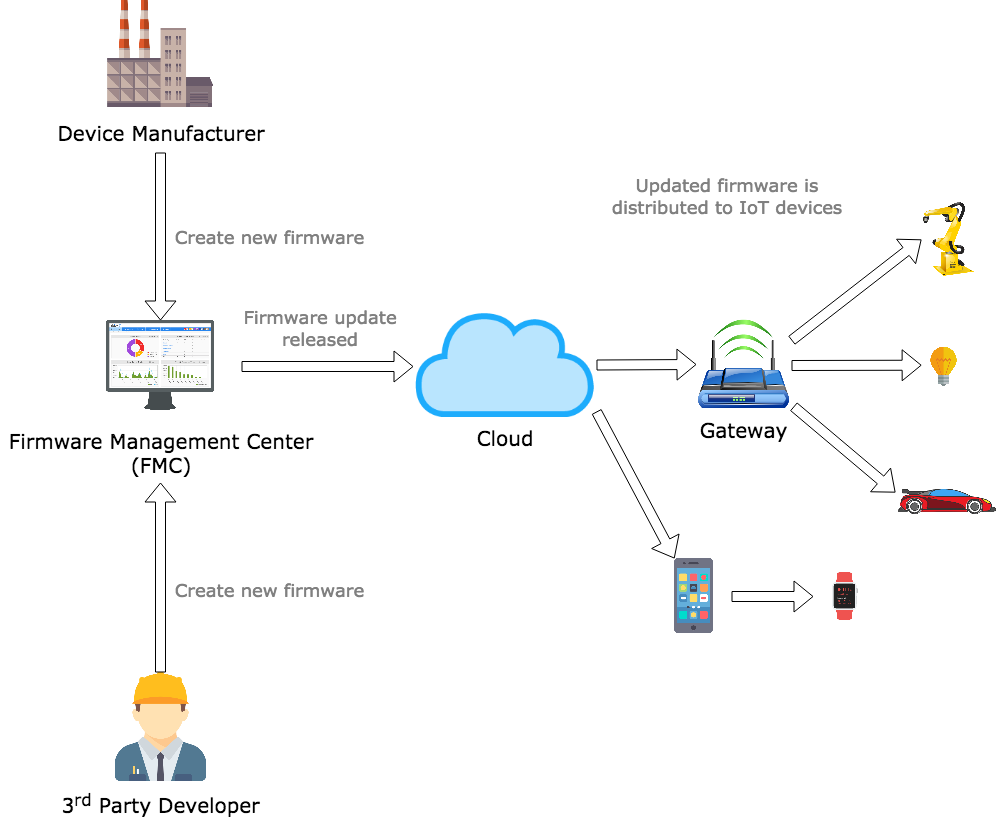
\includegraphics[width=1.0\textwidth]{figures/img_firmware_update_fota.png}
		\caption{Firmware Over The Air (FOTA) process diagram} 
		\label{fig:1_fota}
	\end{center}
\end{figure}

Remote firmware update uses two methods in its process, push and pull method. While push method is applicable for resource constrained device, pull method is more practical for more powerful with stable connection device~\cite{securefota}. Both methods use client-server architecture, in the push method, vendor repository as the server sends the firmware binary as chunks to the device as the client. After receiving the whole firmware binary, client will notify the server aby sending an error or success message. If there is no error, client can do the firmware update. In pull method, vendor repository as a server will provide a url to download the firmware binary to the gateway as the client. Once the whole firmware binary is downloaded, the error or success notification message will be sent back to the server. Then, client can do the firmware update if the download is successful.

\section{Blockchain}
\label{sec:2_blockchain}

Based on Satoshi Nakamoto~\cite{Satoshi}, blockchain was originally created for peer-to-peer electronic cash payment transaction based on cryptographic proof instead of trust (to third party, such as Bank). Satoshi Nakamoto proposes a solution to prevent the double-spending problem in peer-to-peer network without a trusted third party. Each transaction data in the blockchain network is verified, time-stamped and linked with the previous data in the form of chained hash (proof-of-work). By doing so, blockchain technology can create a record that cannot be changed without redoing the hash-based proof-of-work.

Bitcoin's proof-of-work uses Adam Back's Hashcash~\cite{hashcash} which is originally created to limit email spam and denial of service attack (DDoS). The block generation process in Bitcoin uses Hashcash as its proof-of-work. In order for a block to be accepted by network participants, miners must complete a proof-of-work which covers all of the data in the block. Miner is any node that lends their computational resource in order to secure the network and is rewarded with some bitcoin. The first miner who finds the nonce and successfully creates the new block will be rewarded.

Bitcoin implement the proof-of-work ~\cite{proofofwork} by incremental nonce in the block until a value (nonce) is found, this nonce together with the transaction data must give block's hashed value (using SHA-256) the required zero bits. The example of how Bitcoin's proof-of-work iterates nonce is shown in Figure ~\ref{fig:2_proofofwork}. In this example, the required zero value is 3 and it must be in the beginning of the hash value. Total of 4251 hashes iteration is needed in this case, which is not a very hard computation (most computer can achieve at least 4 million hashes per second). That is why Bitcoin automatically varies the difficulty to keep a roughly constant rate of block generation. The difficulty of this proof-of-work is adjusted so as to limit the rate at which a new block can be generated in the network for every 10 minutes. Due to the very low probability of successful generation of a block, this makes it unpredictable which worker computer (miner) in the network will be able to generate the next block.

\begin{figure}[H]
	\begin{center}
		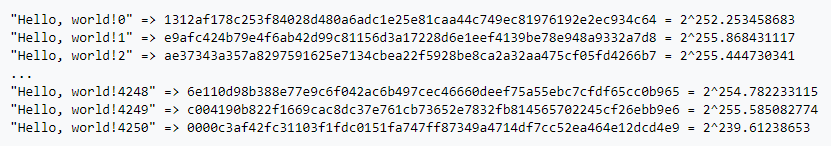
\includegraphics[width=1.0\textwidth]{figures/proofofwork.png}
		\caption{Iterating nonce that make hashes value begin with a number of zero value~\cite{proofofwork}} 
		\label{fig:2_proofofwork}
	\end{center}
\end{figure}

After the correct nonce and its corresponding hash value is found in the mining process, chaining algorithm is depicted in Figure ~\ref{fig:3_blockchainning}. Each block's hash value contains the hash value of previous block. As all blocks in the ledger are chained with its previous block, any modification on the value of any block will affect the whole blocks structure in the network. This mechanism makes blockchain tamper-proofing, means that no one can modify nor tamper a transaction once it is validated and recorded into blockchain.

\begin{figure}[H]
	\begin{center}
		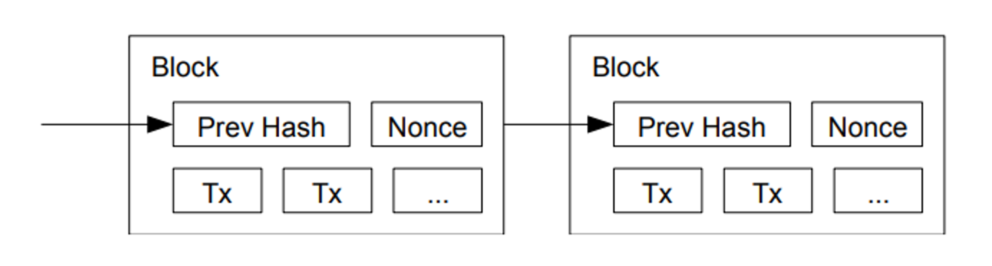
\includegraphics[width=1.0\textwidth]{figures/block-chainning.png}
		\caption{Nakamoto's chaining block diagram~\ref{fig:3_blockchainning}} 
		\label{fig:3_blockchainning}
	\end{center}
\end{figure}

\section{Skiplist}
\label{sec:3_skiplist}

\textit{Skiplist} was first described in 1989 by William Pugh ~\cite{skiplistOriginate}. Skiplist is a data structure that allows fast search within an ordered sequence of elements ~\cite{wiki:skiplist}, fast search is possible by skipping over a few element rather than searching linear number of steps. The structure of a skiplist is shown in Figure ~\ref{fig:4_skipliststructure}. As an example, the search process to find the fifth node, the skiplist firstly traverse a link of width 1 at the top level. Now four more steps are needed, but the next span on this level is too large (10), so it will drop one level to level 3. The algorithm once again traverse one link of width 3. Since the next step of width 2 is skpping too far (becomes 6), instead of traversing in the same level, it will drop down to the bottom level. Lastly the skiplist will traverse the final link of width 1 to reach the fifth link (target).

\begin{figure}[H]
	\begin{center}
		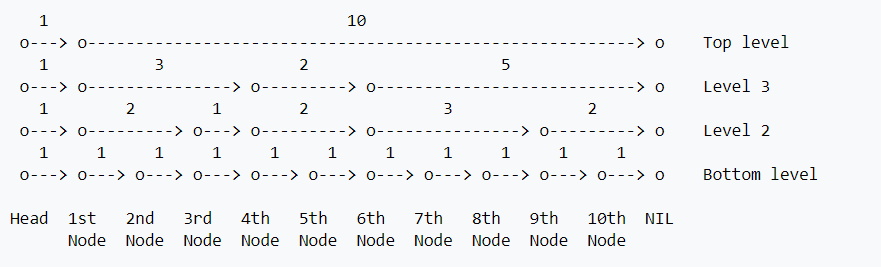
\includegraphics[width=1.0\textwidth]{figures/skiplistSearch.png}
		\caption{Skiplist structure with span between two same-level nodes~\ref{fig:4_skipliststructure}} 
		\label{fig:4_skipliststructure}
	\end{center}
\end{figure}

Based on how the insertion process, there are two types of skiplist. In deterministic skiplist, user needs to define how the insertion process needs to be done. For example J. Ian Munro~\cite{deterministicSkiplist} defined "1-2 skiplist", "1-2 skiplist" structure requires either one or two nodes of height (h-1) exist between any two nodes of height {\emph{h}} ({\emph{h}} > 1). The deterministic skiplist structure is shown at Figure ~\ref{fig:5_deterministicSkiplist}

\begin{figure}[H]
	\begin{center}
		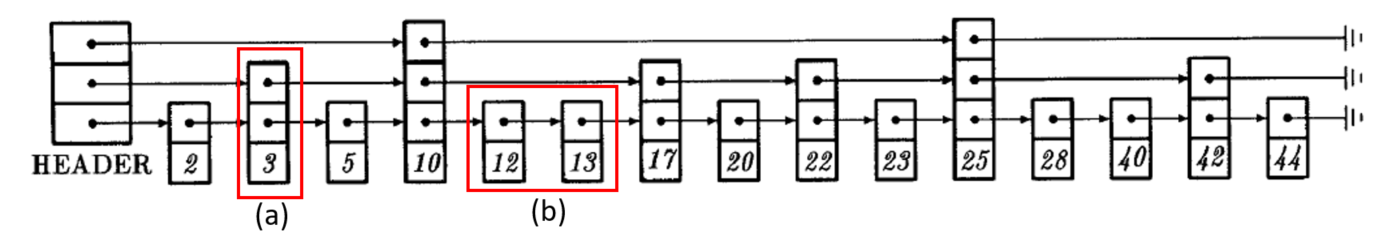
\includegraphics[width=1.0\textwidth]{figures/deterministicSkiplist.png}
		\caption{(a) There is a node with height of two between two nodes with height of three. (b) There are two nodes with height of one between two nodes of height of two~\cite{deterministicSkiplist}} 
		\label{fig:5_deterministicSkiplist}
	\end{center}
\end{figure}

On the other hand, a randomized skiplist defines the new node height based on probabilistic of a coin toss. It will add the height of the newly inserted node until the coin-toss lands on tail or the height reach the maximum-defined-height. The randommess makes the average insert and update cost for the skiplist is low. Randomized skiplist can achieve simple implementation but requires larger storage. 

\section{Skipchain}
\label{sec:4_Skipchain}
One of the key characteristic of blockchain is the traceable asset. It allows all blockchain's participants know where the asset come from and how it change overtime. However, to verify an asset will require user's device to be online, connected to the Internet and to pay bandwidth and power costs to maintain the connectivity with multiple nodes on blockchain network~\cite{Skipchain}. User can to join as a full node, maintaining a mirror copy of the entire blockchain to verify or trace an asset. As an option, user can join as a lightweight node and download partial amount of the entire blockchain data from connected full node. However, it is difficult for low power, limited storage and limited connection device to join the blockchain network even as lightweight node.

Joining a blockchain network as a lightweight node is not without risk, a compromised full node can isolate the connected lightweight node using a "fake" view of blockchain. The lightweight node can do a secure verification by synchronizing with multiple full node, but the compromised full node can achieve it goals by deceiving the isolated lightweight node during the "offline" state. The blockchain node remain vulnerable to isolation attack because the fundamental problem is that the current blockchain can never be validated in any absolute ways, but only relative to the perspective from another node.

To tackle this issue, Chainiac~\cite{chainiac} introduced skipchain, a novel cryptographic blockchain structure that adapts the skiplist idea by adding long-distance links both forward and backward in time as illustrated in Figure ~\ref{fig:6_skipchainStructure}. When Chainiac creates new block, it will create additional hash link to farther backward in time. On the same time, Chainiac also creates long-distance forward link via collective signatures~\cite{cosigning}. With long-distance forward and backward link, skipchain technology becomes cryptographically traversable in both directions. 

\begin{figure}[H]
	\begin{center}
		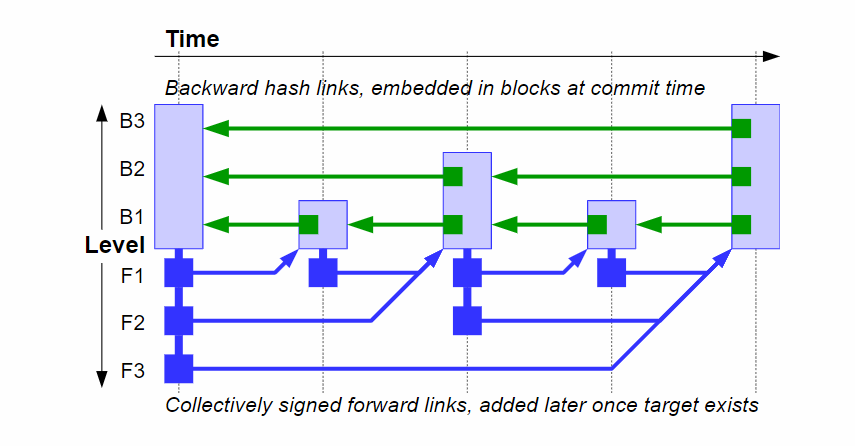
\includegraphics[width=1.0\textwidth]{figures/skipchainStructure.png}
		\caption{Skipchain structure~\cite{chainiac}} 
		\label{fig:6_skipchainStructure}
	\end{center}
\end{figure}

Using this skipchain characteristic, node as a client can efficiently prove the correctness of a transaction anywhere in time with respect to other party reference point on the blockchain, in a logaritmic number of steps, regardless of which node has a more up-to-date data view of the blockchain~\cite{Skipchain}. For example, a gateway in a smart home environment wants to show a new firmware update to a connected IoT device. In this case, the IoT device has limitations to connect to the Internet and to synchronize with the other node. The IoT device can not store partial part of the blockchain data due to its limited storage. The gateway can simply sends to the IoT device a small number of collectively signed forward links through a peer-to-peer connection to prove securely that the new firmware updates is indeed on the blockchain. 

\section{Blockchain-based Firmware Update Framework}
\label{sec:5_proposedFramework}

In this section, previous researches on the firmware update mechanism for embedded devices based on blockchain infrastructure are introduced. Lee et al.~\cite{lee} introduced the blockchain-based firmware verification and update schemes for embedded devices in IoT environment. Lee et al. mentioned that excessive network traffic may occur when large number of embedded devices downloading the latest firmware simultaneously from a dedicated firmware update server. This problem leads Lee et al. to utilize blockchain network concept, where a device can request a firmware update from a decentralized peer-to-peer network.

\sloppy In~\cite{lee} architecture, embedded device acted as full node in the blockchain network which was difficult to be implemented in real world scenario. Because the embedded devices with low-power, limited storage and limited connection to the Internet are difficult to maintain connection with the other node in blockchain network. It is also not possible for the embedded device to store growing blockchain data. Moreover, when there are many kind of embedded device with different requirement of firmware, it will take a long time to make the download request because this scheme used pull-method. In result, this scheme might not efficient for heterogeneous IoT ecosystem.

Boudguiga et al.~\cite{boudguiga} investigated that it was possible to use blockchain infrastructure to provide firmware update to several embedded devices belonging to different manufacturer. This scheme relied on trusted node in the blockchain to validate an update innocuousness before its transmission to the end objects. The trusted node checks that the new update does not contain bugs and resist to known attack.

There are two architectures introduced by~\cite{boudguiga}. In the first architecture, each vendor was expected to provide at least one worker node in the blockchain network. An embedded device could periodically pull the blockchain by random picks the node and check the firmware version. The mentioned trusted node takes place in the second architecture as a refinement from the first architecture. The trusted node directly receives new firmware binary from the vendor, then notifies the corresponding embedded devices after the validation process completed. The corresponding device can download the valid firmware binary and do the firmware update.

	% \chapter{System Environment and Protocol Designs}
\label{cha:3_design}
\parskip=0ex

\indent This chapter describes the assumptions used in this thesis, an overview on Skipchain technology, the proposed system architecture design and the proposed protocol design. All assumptions used in the proposed firmware update framework is described in Section~\ref{sec:1_assumptions}. An overview of Skipchain technology is explained in Section~\ref{sec:2_overview}. The system architecture design and the proposed protocol design for the firmware update mechanism are explained in Section~\ref{sec:3_architectureDesign} and Section~\ref{cha:4_protocoldesign}, respectively.

\section{Assumptions}
\label{sec:1_assumptions}

The assumptions used in this thesis are listed as follows:
\begin{enumerate}
	\item The proposed firmware update mechanism uses push-update method, in which the vendor repository sends the metadata of a new firmware in the form of smart contract to the skipchain network. Once the corresponding smart contract is verified, all the nodes in the skipchain network will synchronize their smart contract data with the latest data.
	\item  In the proposed scenario, the gateway as a passive node in the skipchain network will obtain a notification on the newly released firmware from the verified smart contract. Afterward, the gateway will check if the newly released firmware is required by the IoT devices connected to it.
	\item The scope of IoT devices in this thesis have low-power consumption, small storage capacity, limited computation capability, and limited Internet connectivity. However, the IoT devices are able to perform simple Hash computation and simple value comparison.
	\item The IoT devices have pre-installed the public key of vendor to authenticate the firmware signature.
	\item Each IoT device have pre-installed a small portion of skipchain data to allow the associated gateway to join a specific skipchain network. In addition, the pre-installed skipchain data enable the IoT device to securely verify the more recent skipchain data from the associated gateway.
	\item The firmware binary is distributed from the vendor repository to the targeted IoT device through a secure channel.
	\item The vendor repository and the corresponding vendor node are communicating through a non-secure communication channel.
	\item The peer-to-peer connection between gateway and IoT devices is not in secure channel.
\end{enumerate}

\section{Skipchain Overview}
\label{sec:2_overview}

Skipchain is a cryptographically traversable, offline and p2p verifiable blockchain structure~\cite{Skipchain}. Skipchain implements the concept of skiplist into a blockchain structure by adding long-distance forward and backward links. The long-distance backward link has been introduced in Chainiac~\cite{chainiac}. The long-distance backward link contains a hashed-address of the previously created block. This backward link allows users to trace a transaction history starting from the latest block data. The transaction trace feature could be performed when the user's device contains more recent block data than the block data of searched transaction.

The unique forward link in skipchain structure enables user to verify transaction history even when the user's blockchain data is behind the more recent blockchain data. This forward link contains two pieces of information as follow:
\begin{enumerate}
	\item A secure hash-pointer to the first block committed by the next consensus group.
	\item A description of how the consensus group has changed, such as which cosigner joins or leaves the consensus group (indicated by the addition or reduction on the number of cosigner's public keys).
\end{enumerate}
Once the successor of a block is committed, the consensus group responsible for the block creates and collectively signs a forward link. This process is similar to securely issues an information of the current consensus group's members for the prior, already-committed block. The security of forward link is assured by a collective signature.

Skipchain uses a tree-based collective signing (CoSi)~\cite{cosigning} schemes, in which each signer (\textit{cosigner}) joins the Schnorr signature~\cite{schnorrsign} to agree on a valid statement. The group of cosigner, known as collective authority (cothority), will perform the consensus-like process where each cosigner will verify and sign a valid transaction. The CoSi architecture is illustrated in Figure~\ref{fig:cothority}. In the CoSi architecture, each record could be collectively signed by different cothority member.
\begin{figure}[H]
	\begin{center}
		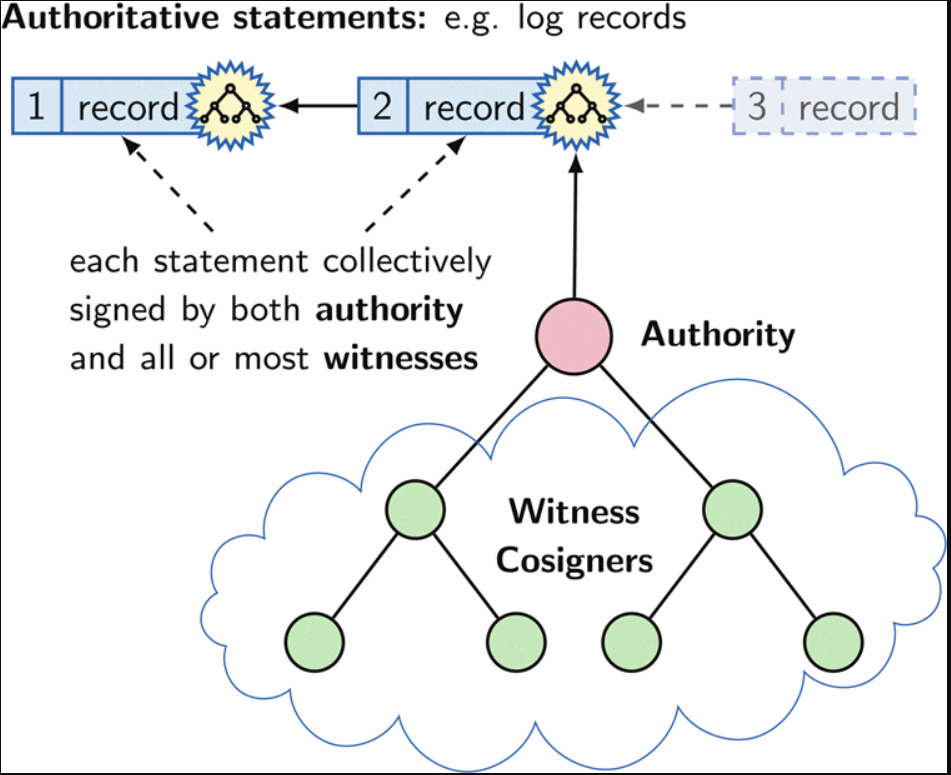
\includegraphics[width=1.0\textwidth]{figures/cosigning.png}
		\caption{CoSi protocol architecture~\cite{cosigning}} 
		\label{fig:cothority}
	\end{center}
\end{figure}

As the forward links are signed by different cothority members, the user could securely perform forward tracing on the more recent blockchain data without having to trust the other parties. In addition, the user could learn all the changes on the consensus group and would be able to know the correct set of public keys while performing the forward tracing. The set of public keys will be used to verify the corresponding collective signatures in the blockchain. Since all of the forward links are collectively signed by cothority members, an attacker can not create a fake blockchain branch unless the attacker compromises or colludes with large number of cothority members.

\section{Architecture Design}
\label{sec:3_architectureDesign}

In this thesis, we proposed the skipchain-based firmware update framework for IoT environments. The architecture of our framework is illustrated in Figure~\ref{fig:1_fotb}. There are three roles in the architecture design, described as follow:
~\begin{enumerate}
	\item Vendor: the manufacturer of the specific IoT device and acts as active node in the skipchain network. The active node in the skipchain network is actively do the verification process as a Cothority's member. Each time a vendor pushes a new version of firmware, the vendor repository needs to broadcast the vendor-signed firmware metadata to the Cothority nodes via the vendor's active node.
	\item Gateway: the gateway for connected IoT devices and connected to the skipchain network as passive node. The passive node in skipchain network does not participate in any verification process, however, it only synchronizes the block data with the most recent block data in the skipchain network.
	\item IoT device: the sensor-embedded device that connects to a specific gateway and does not need to fully trust the gateway device. Each IoT device can verify the notification of firmware update from the gateway by using its pre-installed skipchain data.
\end{enumerate}

\begin{figure}[H]
	\begin{center}
		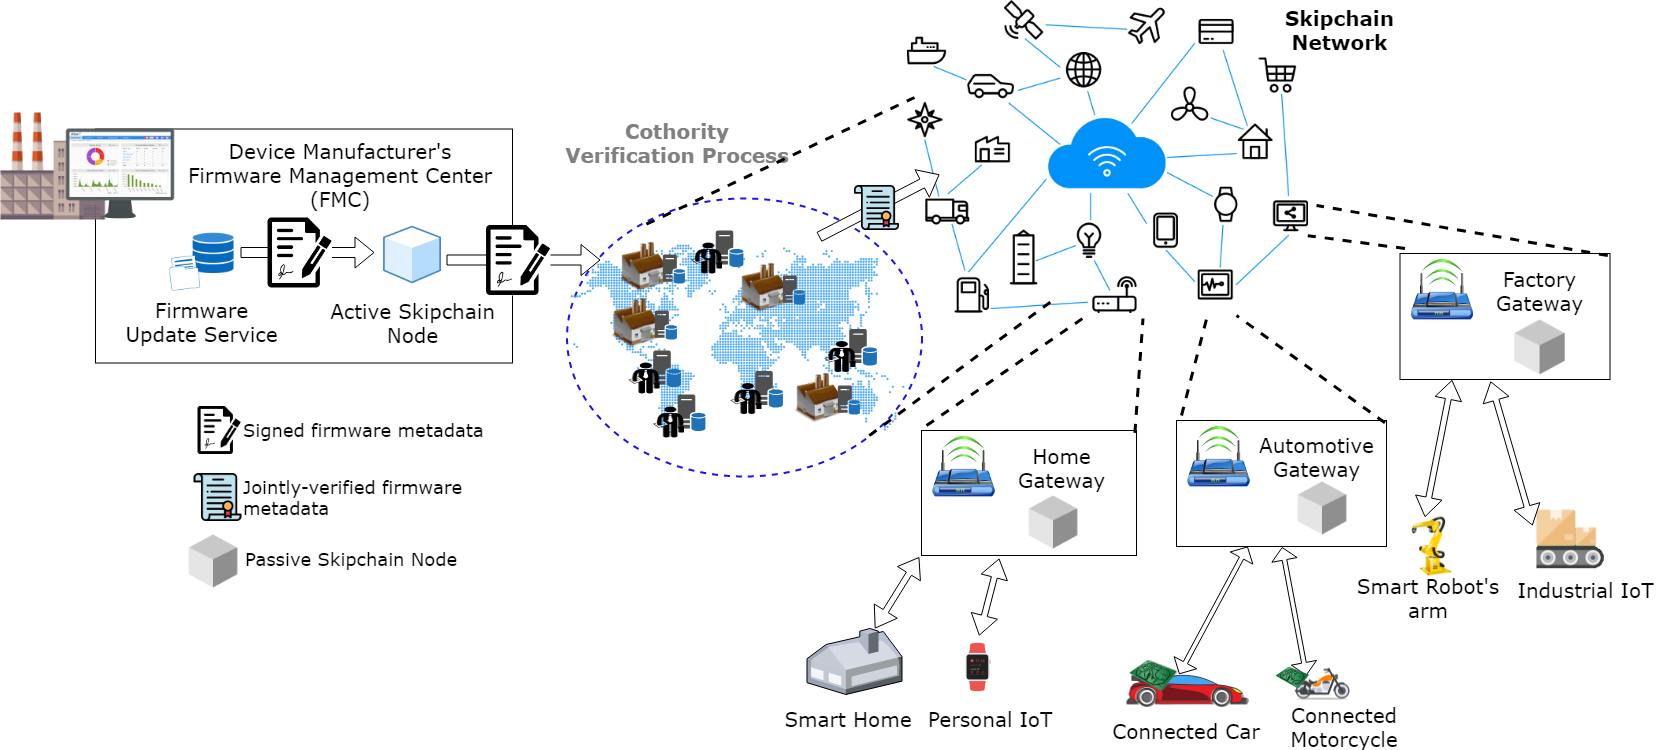
\includegraphics[width=1.0\textwidth]{figures/firmware_update-skipchain-based_fotb.png}
		\caption{Firmware Over-the-Skipchain (FOTS) process diagram} 
		\label{fig:1_fotb}
	\end{center}
\end{figure}

From the Figure~\ref{fig:1_fotb}, there are two kinds of node in the skipchain network namely: active node and passive node. The active nodes are actively performing the verification process on any new smart contract data containing the metadata of a new version of firmware. In addition, the active node acts as Cothority's member in the proposed skipchain network. In the contrary to the active node, the passive node only continuously synchronizes the block data with the more recent block data in the skipchain network and does not involve in any verification process of a newly released smart contract. Each gateway in the proposed architecture design manages at least one IoT device in local network environment. For example, there are smart home appliances and personal IoT devices connected to a home router as gateway. The connection between the gateway and the IoT device is peer-to-peer connection, such as Bluetooth connection.

\begin{figure}[H]
	\begin{center}
		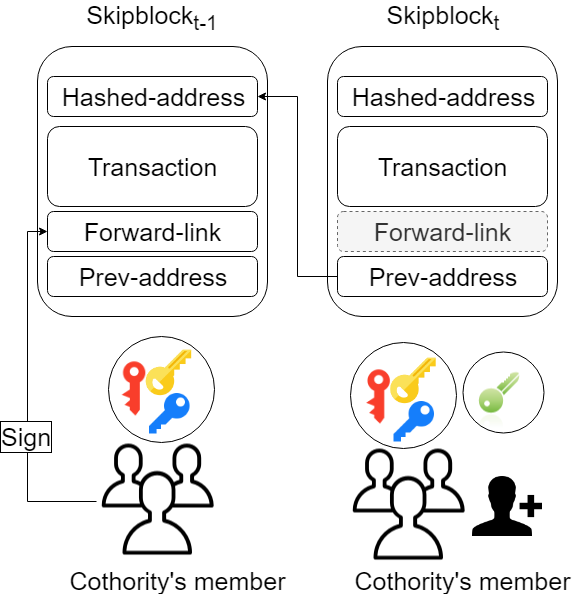
\includegraphics[width=1.0\textwidth]{figures/firmware_update-skipblock-diagram.png}
		\caption{Skipblock structure diagram} 
		\label{fig:skipblock_diagram}
	\end{center}
\end{figure}

The skipblock structure as shown in Figure~\ref{fig:skipblock_diagram}, consists of four main contents: hashed-address, transaction, forward link, and prev-address. These four contents are described as follow:
~\begin{enumerate}
	\item Hashed-address: a hashed-value that is unique and will be the address for a skipblock. Each skipblock is accessible through this hashed-address.
	\item Transaction: the transaction contains the metadata of a firmware, such as the targeted device model, the firmware version, and the url to download the corresponding firmware binary in the vendor repository. A skipblock could contain one or more transaction data.
	\item Forward Link: the unique structure from skipchain itself, it contains the next block's address and the difference of the current cothority's members that verify the $skipblock_t$. The cothority's members those verify the $skipblock_{t-1}$ (red, yellow and blue key) need to sign the forward link. In Figure~\ref{fig:skipblock_diagram}, the forward link will contain the information about the new cothority's member with the green key. Later, client will check the forward link, and know which keys do the client need to use to verify the skipblock. And the dashed-line forward link in $skipblock_t$ means that it contain no information of the next block since $t$ is the newest block.
	\item Prev-address: the hashed-address of a previous skipblock.
\end{enumerate}

\begin{figure}[H]
	\begin{center}
		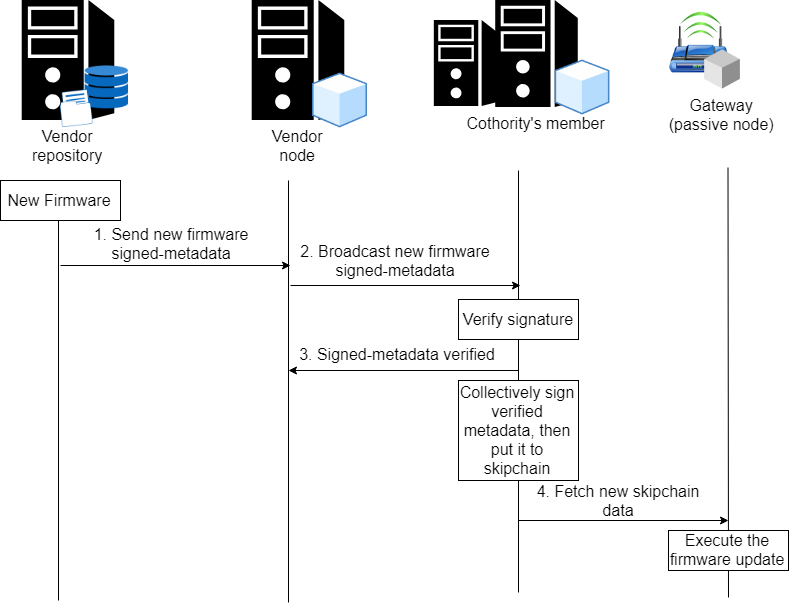
\includegraphics[width=1.0\textwidth]{figures/firmware_update-Firmware_verification_process.png}
		\caption{Firmware update verification process} 
		\label{fig:verificationprocess}
	\end{center}
\end{figure}

In our proposed scheme, we divide the overall process into two parts. The first part is firmware verification process, in which this process will leverage how the metadata of a new version of firmware is verified and how to store the corresponding metadata into the skipchain. After the metadata of the corresponding firmware is sent to the skipchain network, the peer-to-peer verification process will begin. Afterward, the IoT device verifies the firmware update notification from the gateway (in a peer-to-peer connection) before the firmware update is performed by the IoT device.

The firmware verification process of the proposed framework is shown in Figure~\ref{fig:verificationprocess} and described as follow:
~\begin{enumerate}
	\item Each time a vendor releases a new version of firmware, the vendor uses his private key to sign the metadata of the newly released firmware. The metadata of a firmware contains information such as the url to download the corresponding firmware, the version of a firmware, the targeted device model, and other detailed information which will be discussed in Section~\ref{cha:4_protocoldesign}.
	\item The vendor node broadcasts the signed-metadata to the other cothority member to be verified using the corresponding vendor's public key.
	\item After the verification process for the firmware metadata, the cothority will collectively sign the valid metadata and store the signed firmware metadata into the skipblock in the skipchain network.
	\item The gateway as a passive node will continuously synchronize with the skipchain network to fetch the new firmware update information and execute the firmware update mechanism.
\end{enumerate}

The firmware update peer-to-peer verification process is illustrated in Figure~\ref{fig:executionprocess}. After obtaining the firmware update notification, the gateway checks the targeted device model for the firmware update from the newly created skipblock. Afterward, the gateway will notify the corresponding connected IoT devices. Then, the IoT device can verify if the updated firmware comes from the valid skipblock and whether the firmware is published by the correct vendor. After the updated firmware is verified, the IoT device sends its current firmware version to the gateway. Upon receiving the installed firmware version from the IoT device, the gateway will check whether the installed version of firmware is older than the new version of firmware recorded in the skipblock. In the case that the installed firmware version in the IoT device is older than the firmware version in the skipblock, then the gateway will download the new version of firmware binary from the url provided in the metadata. The downloaded firmware binary is sent to the corresponding IoT device to be verified and installed to the device.

\begin{figure}[H]
	\begin{center}
		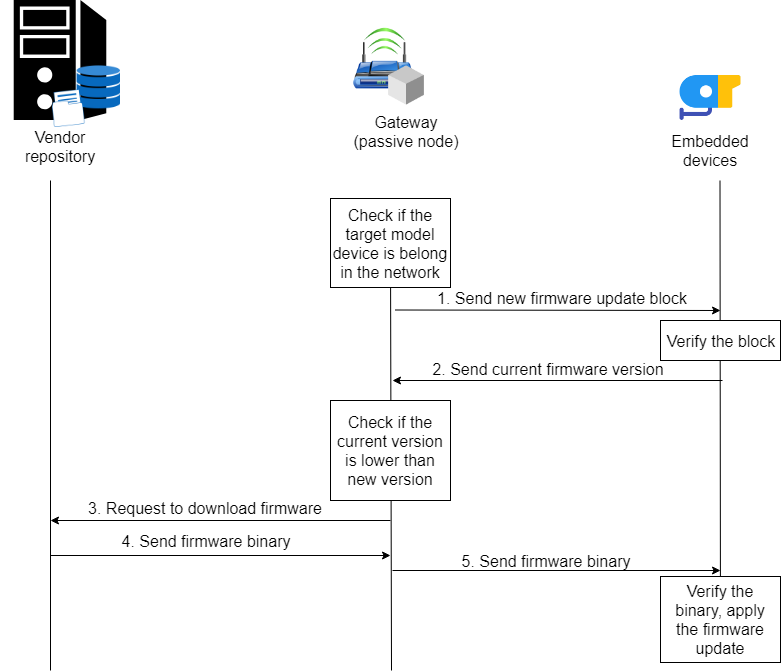
\includegraphics[width=1.0\textwidth]{figures/firmware_update-firmware_update_execution.png}
		\caption{Firmware update peer-to-peer verification process} 
		\label{fig:executionprocess}
	\end{center}
\end{figure}

In the peer-to-peer verification process, the IoT device uses the skipchain's forward link to securely verify the new version of firmware without synchronizing and storing any additional data. Instead, the gateway as a more capable device with more storage capacity and more stable Internet connection can do the synchronization process. The peer-to-peer verification also helpful when a gateway is not connected to the Internet because the offline-gateway can get the firmware update notification from another online-gateway via peer-to-peer notification. In such case, the offline-gateway is still able to verify the new firmware update notification and does not blindly trust the online-gateway. The peer-to-peer verification process is illustrated in Figure~\ref{fig:p2pverification}

\begin{figure}[H]
	\begin{center}
		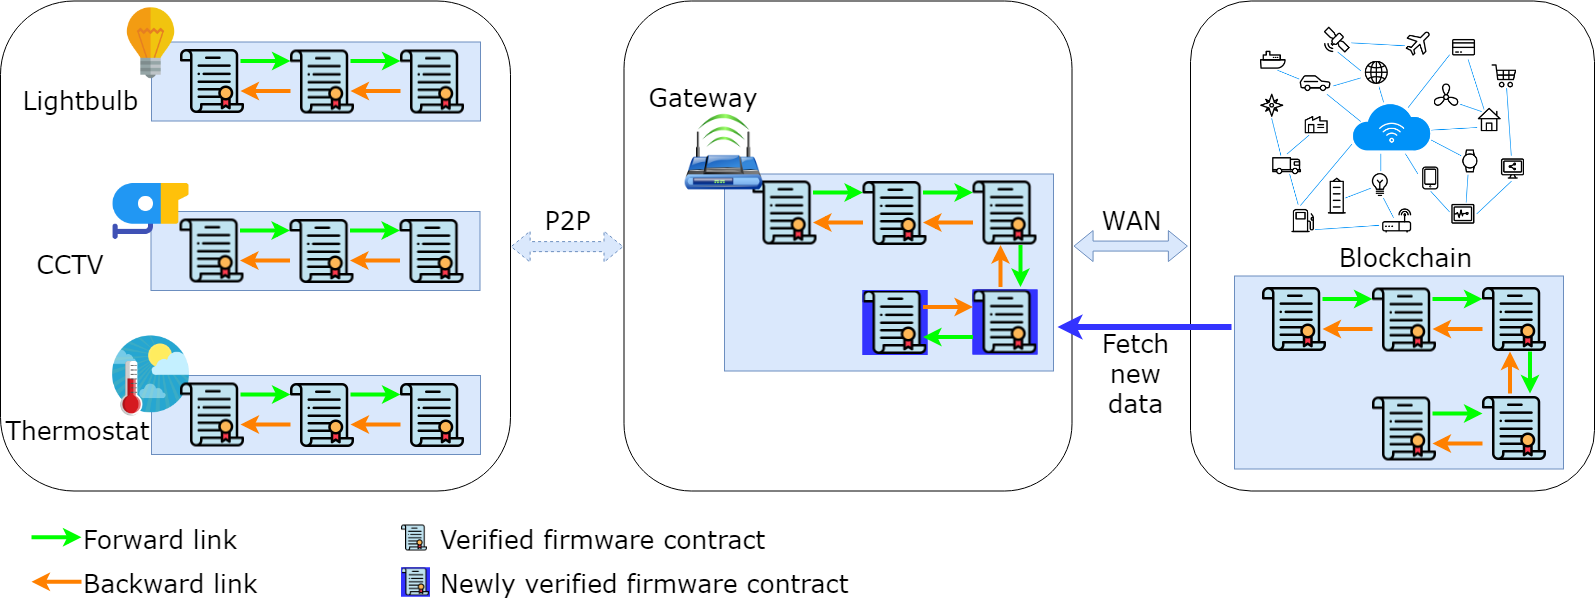
\includegraphics[width=1.0\textwidth]{figures/firmware_update-skipchain_p2p_update.png}
		\caption{Peer-to-peer verification process} 
		\label{fig:p2pverification}
	\end{center}
\end{figure}

In the peer-to-peer verification process, the pre-installed skipblock in the IoT device takes an important role as it contains several valid skipblocks data. The pre-installed skipblock structure is illustrated in Figure~\ref{fig:preinstalled}. In addition, the pre-installed skipblocks contain list of public keys (illustrated by the red, yellow and blue keys in the Figure~\ref{fig:preinstalled}) to verify the given forward link via peer-to-peer connection.

\begin{figure}[H]
	\begin{center}
		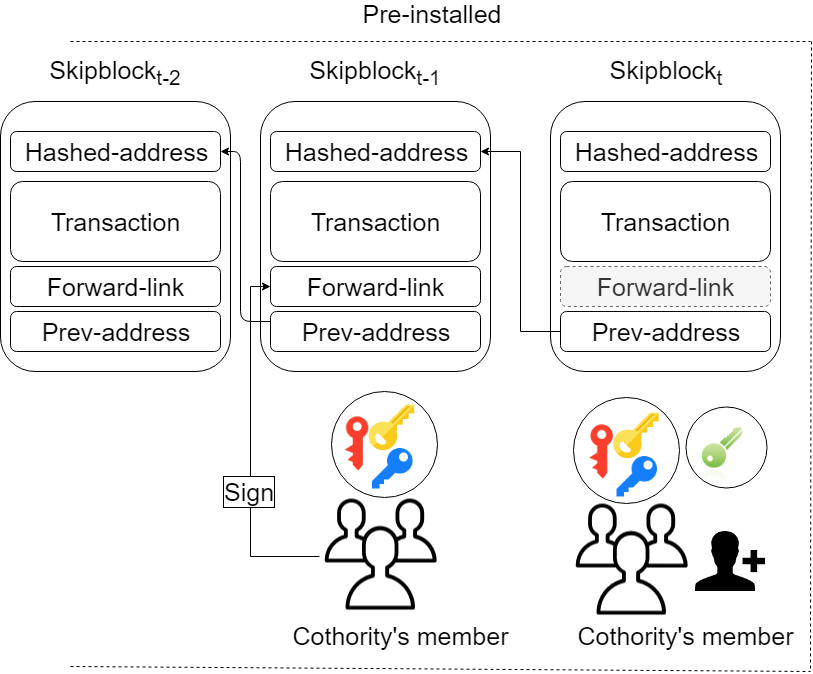
\includegraphics[width=1.0\textwidth]{figures/firmware_update-preinstalled_skipblock.png}
		\caption{Pre-installed skipblock diagram} 
		\label{fig:preinstalled}
	\end{center}
\end{figure}

\section{Protocol Design}
\label{cha:4_protocoldesign}

In this section, our proposed firmware update protocol is introduced and explained. There are two stages of verification before the firmware binary is executed in the proposed protocol: firmware update verification process and peer-to-peer verification process between IoT device and gateway. Table \ref{tab:notation} shows the notations that we use in our protocol.

\begin{table}[H]
	\caption{Notation used in the proposed protocol}
	\label{tab:notation}
	\begin{center}
		\begin{tabular}{cl}
			\hline
			\textbf{Notation} & \multicolumn{1}{c}{\textbf{Definition}} \\ \hline
			\boldmath{$ID_{d}$} & The unique ID of an IoT device \textit{d} \\
			\boldmath{$ID_{g}$} & The unique ID of a gateway \textit{g} \\
			\boldmath{$ID_{v}$} & The unique ID of a vendor \textit{v} \\
			\boldmath{$ID_{b}$} & The unique ID of a skipblock \textit{b} \\
			\boldmath{$ID_{c}^{v}$} & The unique ID of cosigner node \textit{c} owned by a vendor \textit{v} \\
			\boldmath{$k$} & The session key \\
			\boldmath{$sid$} & The unique ID of a specific session \\
			\boldmath{$p$} & Randomly generated shared prime number in key exchange process\\
			\boldmath{$g$} & Shared base number in key exchange process\\
			\boldmath{$s$} & Shared secret between key exchange process\\
			\boldmath{$a,b$} & Secret owns by Alice and Bob in key exchange process\\
%		\end{tabular}
%	\end{center}
%\end{table}
%\begin{table}[H]
%	\label{tab:notation2}
%	\begin{center}
%		\begin{tabular}{cl}
%\begin{tabular}{l@{}l@{}}The key derivation function. The inputs of this function are passphrase and salt \\and the output of this function is a session key \textit{k}\end{tabular}
%			\hline
%			\textbf{Notation} & \multicolumn{1}{c}{\textbf{Definition}} \\ \hline
			\boldmath{$URL_d^v$} & \begin{tabular}{l@{}l@{}}The url to download the corresponding firmware binary for the targeted \\IoT device \textit{d} from a specific vendor \textit{v}\end{tabular}\\
			\boldmath{$CFV_d^v$} & The current firmware version installed in the IoT device \textit{d} from vendor \textit{v}\\
			\boldmath{$LFV_d^v$} & The latest firmware version for IoT device \textit{d} from vendor \textit{v}\\
			\boldmath{$LFB_d^v$} & The latest firmware binary for IoT device \textit{d} from vendor \textit{v}\\
			\boldmath{$M_d^v$} & The device model for targeted IoT device \textit{d} from vendor \textit{v}\\
			\boldmath{$BLOCK_s$} & The pre-installed skipchain \textit{s} block from the vendor\\
			\boldmath{$BLOCK_t$} & The skipchain block in newest timestamp \textit{t}\\
			\boldmath{$KDF()$} & \begin{tabular}{l@{}l@{}}The key derivation function. The inputs of this function are passphrase and salt \\and the output of this function is a session key \textit{k}\end{tabular} \\
			\boldmath{$E_k()$} & Symmetric key encryption using session key \textit{k}\\
			\boldmath{$D_k()$} & Symmetric key decryption using session key \textit{k}\\
			\boldmath{$H()$} & One-way hash-chain function\\
			\boldmath{$||$} & String concatenation operation\\
		\end{tabular}
	\end{center}
\end{table}

\subsection{Firmware Update Verification Protocol}
\label{sec:verificationprotocol}

\indent This verification protocol is initiated each time a vendor (\textit{v}) has new updated firmware to be published in the skipchain network (\textit{$URL_s$}). This protocol is running under the assumption that the connection between the vendor repository and vendor node (as cothority's member) is not secure. Cothority will do the consensus-like verification protocol before a new block (\textit{$BLOCK_t$}) is created. Vendor node will broadcast the new firmware update metadata to each cothority member, then each member will verify the signed-metadata. Vendor node will collect the signature of cothority member, then put the metadata into the new block (\textit{$BLOCK_t$}). Figure \ref{fig:verificationprocessprotocol} shows the firmware update verification protocol.

\begin{figure}[H]
	\begin{center}
		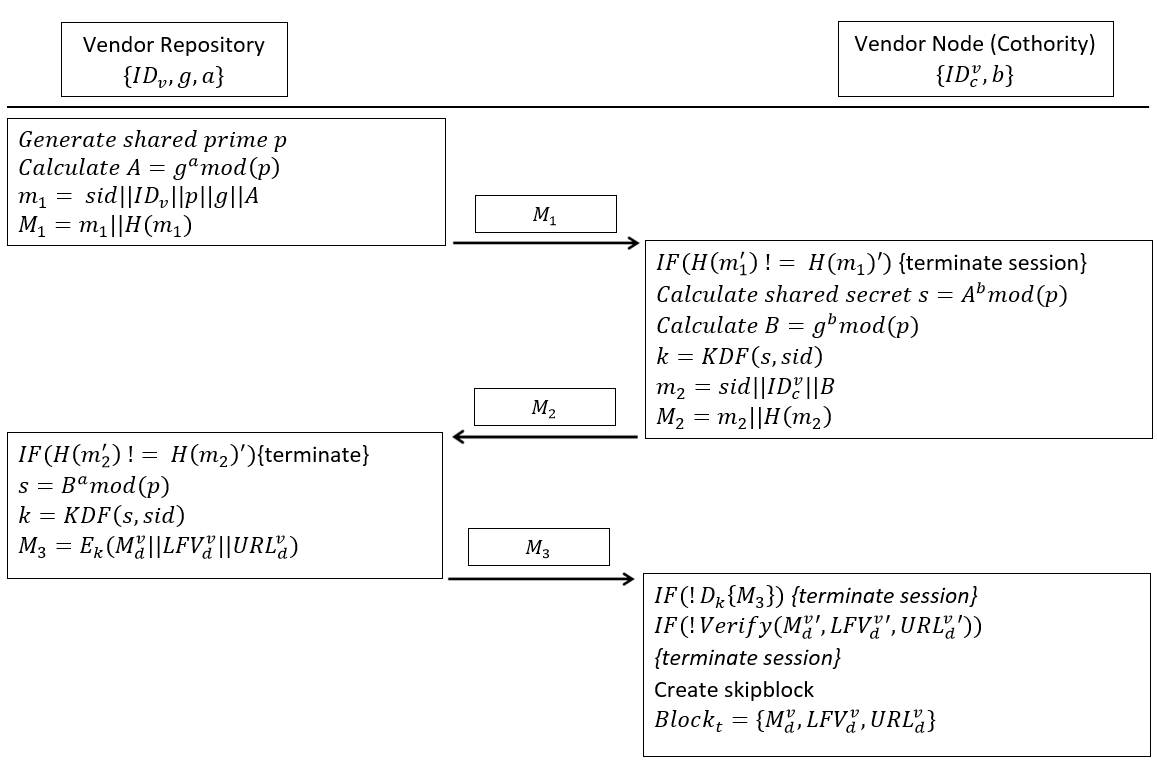
\includegraphics[width=1.0\textwidth]{figures/verification_process_protocol.png}
		\caption{Firmware update verification protocol} 
		\label{fig:verificationprocessprotocol}
	\end{center}
\end{figure}

\noindent \underline{\textbf{Step 1:}} $\text{Vendor Repository}\rightarrow\text{Vendor Node}$ \\
\indent Vendor repository \textit{v} will generate a shared prime \textit{p}, and calculate a shared number \textit{$A=g^a mod(p)$}. This shared number later will be used by vendor node to generate same shared secret. Vendor repository then create a message \textit{$m_1=(sid||ID_v||p||g||A)$}, then concatenate the message \textit{$m_1$} with the hash value of the message \textit{$H(m_1)$} and send it to the vendor node.

\noindent \underline{\textbf{Step 2:}} $\text{Vendor Node}\rightarrow\text{Vendor Repository}$ \\
\indent After receiving message \textit{$m_1'$} from vendor repository, vendor node will validate the message by applying the same hash function \textit{$H()$} to the message \textit{$m_1'$}. If the hashed-value do not match \textit{$H(m_1)'$}, vendor node will terminate the session. Once validated (\textit{$H(m_1')==H(m_1)'$}), vendor node will obtain session id \textit{sid'}, vendor repository's ID \textit{$ID_v'$}, shared prime \textit{p'}, shared base \textit{g'}, and shared number \textit{A'}. Next, vendor node calculate shared secret \textit{$s=A'^bmod(p')$} and shared number \textit{$B=g'^bmod(p')$}. Vendor node uses key derivation function \textit{$KDF()$}, passing shared secret \textit{$s$} and session id \textit{$sid$} as salt to create new session key \textit{$k$}. Vendor node then create a message \textit{$m_2=(sid||ID_c^v||B)$}, then concatenate the message \textit{$m_2$} with the hash value of the message \textit{$H(m_2)$} and send it to the vendor repository.

\noindent \underline{\textbf{Step 3:}} $\text{Vendor Repository}\rightarrow\text{Vendor Node}$ \\
\indent Once receive \textit{$m_2'$}, vendor repository will do the validation toward the message \textit{$m_2'$} and hashed-value \textit{$H(m_2)'$}. If the message is valid (\textit{$H(m_2')==H(m_2)'$}), vendor repository will obtain session id \textit{sid'}, vendor node's id \textit{$ID_c^{v'}$} and shared number \textit{B'} then calculate shared secret \textit{$s=B'^amod(p)$}. It will also use KDF to create same session key \textit{$k$}. Last, vendor repository encrypt message \textit{$m_3=E_k(M_d^v||LFV_d^v||URL_d^v)$} using symmetric encryption protocol with session key \textit{$k$}, then send the message \textit{$m_3$} back to vendor node.

\noindent \underline{\textbf{Step 4:}} $\text{Vendor Node}\rightarrow\text{Vendor Repository}$ \\
\indent Vendor node will decrypt the encrypted message \textit{$m_3'$} using its session key \textit{$k$}, and obtain the new firmware update metadata. Vendor node will broadcast the metadata to cothority member to be verified. Once the verifying process is done, vendor node will collect the signature from participated cothority member. The collected signature proof that the metadata has already verified, and ready to be put in the new skipchain block \textit{$BLOCK_t$}.

\subsection{Firmware Update Peer-to-Peer Verification Protocol}
\label{sec:p2pverificationprotocol}

Peer-to-peer verification protocol occurs between gateway \textit{$g$} and its belonging IoT device \textit{$d$}. This process is needed everytime gateway fetch new block data from the skipchain network (\textit{$URL_s$}). Each IoT device can verify if the firmware update notification from the gateway comes from a valid block from valid a skipchain network. The peer-to-peer verification protocol is shown in Figure \ref{fig:executionprocessprotocol1}.

\begin{figure}[H]
	\begin{center}
		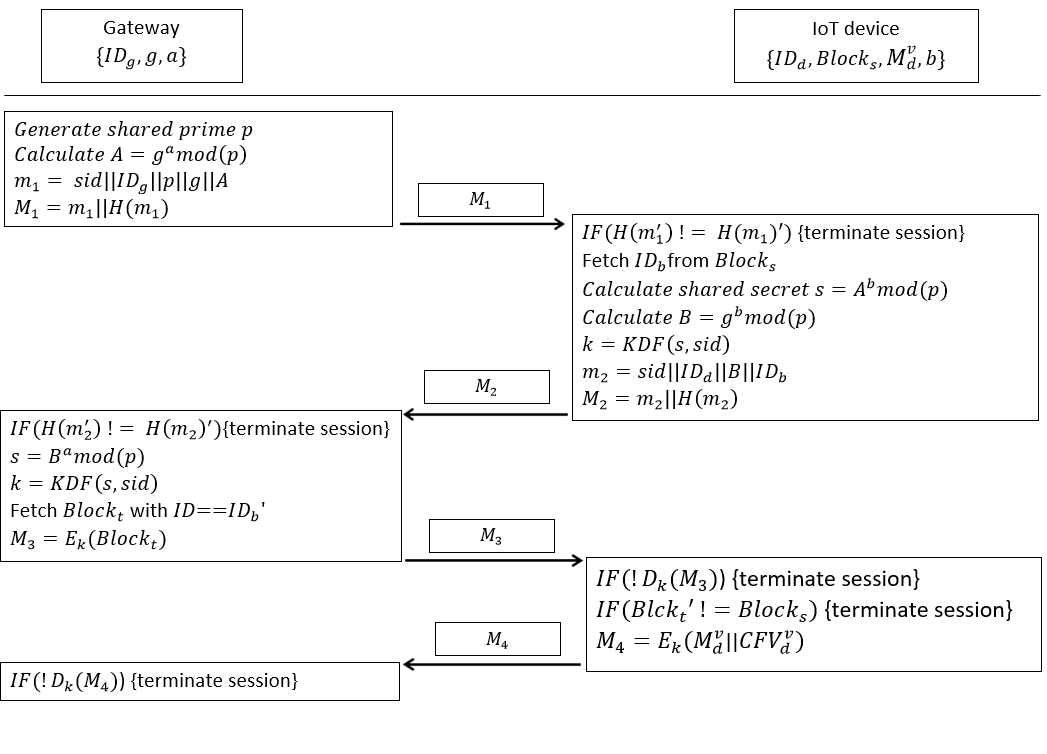
\includegraphics[width=1.0\textwidth]{figures/firmware_update_execution_1.png}
		\caption{Firmware update peer-to-peer verification protocol} 
		\label{fig:executionprocessprotocol1}
	\end{center}
\end{figure}

\noindent \underline{\textbf{Step 1:}} $\text{Gateway}\rightarrow\text{IoT Device}$ \\
\indent Gateway will generate a shared prime \textit{p}, and calculate a shared number \textit{$A=g^a mod(p)$}. Gateway then create a message \textit{$m_1=(sid||ID_v||p||g||A)$}, then concatenate the message \textit{$m_1$} with the hash value of the message \textit{$H(m_1)$} and send it to the IoT device.

\noindent \underline{\textbf{Step 2:}} $\text{IoT Device}\rightarrow\text{Gateway}$ \\
\indent Upon received message \textit{$m_1'$} from gateway, IoT device will validate the message by applying the same hash function \textit{$H()$} to the message \textit{$m_1'$}. If the hashed-value do not match \textit{$H(m_1)'$}, vendor node will terminate the session. Once validated (\textit{$H(m_1')==H(m_1)'$}), vendor node will obtain session id \textit{sid'}, gateway's id \textit{$ID_g'$}, shared prime \textit{p'}, shared base \textit{g'}, and shared number \textit{A'}. Next, IoT device calculate shared secret \textit{$s=A'^bmod(p')$} and shared number \textit{$B=g'^bmod(p')$}. IoT device uses key derivation function \textit{$KDF()$}, passing shared secret \textit{$s$} and session id \textit{$sid$} as salt to create new session key \textit{$k$}. IoT device then create a message \textit{$m_2=(sid||ID_d||B||ID_b)$}, then concatenate the message \textit{$m_2$} with the hash value of the message \textit{$H(m_2)$} and send it to the gateway.

\noindent \underline{\textbf{Step 3:}} $\text{Gateway}\rightarrow\text{IoT Device}$ \\
\indent Once receive \textit{$m_2'$}, gateway will do the validation toward the message \textit{$m_2'$} and hashed-value \textit{$H(m_2)'$}. If the message is valid (\textit{$H(m_2')==H(m_2)'$}), vendor repository will obtain session id \textit{sid'}, IoT device's id \textit{$ID_d^{v'}$}, skipblock id \textit{$ID_b'$} and shared number \textit{B'} then calculate shared secret \textit{$s=B'^amod(p)$}. It will also use KDF to create same session key \textit{$k$}. Gateway fetches the \textit{$BLOCK_t$} with id equals to \textit{$ID_b'$}. Last, gateway encrypt message \textit{$m_3=E_k(BLOCK_t)$} using symmetric encryption protocol with session key \textit{$k$}, then send the message \textit{$m_3$} back to IoT device.

\noindent \underline{\textbf{Step 4:}} $\text{IoT Device}\rightarrow\text{Gateway}$ \\
\indent IoT device will decrypt the encrypted message \textit{$m_3'$} using its session key \textit{$k$}, and obtain the new firmware update block. IoT device will verify the obtained \textit{$BLOCK_t'$} if it is matched with its pre-installed block \textit{$BLOCK_s$}. Once verified, IoT device encrypt its model information and current firmware version it has \textit{$m_4=E_k(M_d^v||CFV_d^v)$} using session key \textit{$k$}. Last, IoT device will send the message \textit{$m_4$} to the gateway.

\noindent \underline{\textbf{Step 5:}} \\
\indent Gateway will decrypt the message \textit{$m_4'$} and obtain model information \textit{$M_d^{v'}$} and current firmware version \textit{$CFV_d^{v'}$} of the IoT device \textit{d}. These information will be used for the next process, the firmware execution protocol in Section \ref{sec:executionprotocol}.

\subsection{Firmware Update Execution Protocol}
\label{sec:executionprotocol}

The firmware update execution will be processed once the peer-to-peer verification process is done. This process uses some variables collected from the peer-to-peer verification process, like session key \textit{$k$}, device model information \textit{$M_d^{v'}$} and device current firmware version \textit{$CFV_d^{v'}$}. With our assumption in Section \ref{sec:1_assumptions}, the IoT device will verify the firmware binary using its pre-installed public key of its vendor. The firmware update execution protocol is shown in Figure \ref{fig:executionprocess}.

\begin{figure}[H]
	\begin{center}
		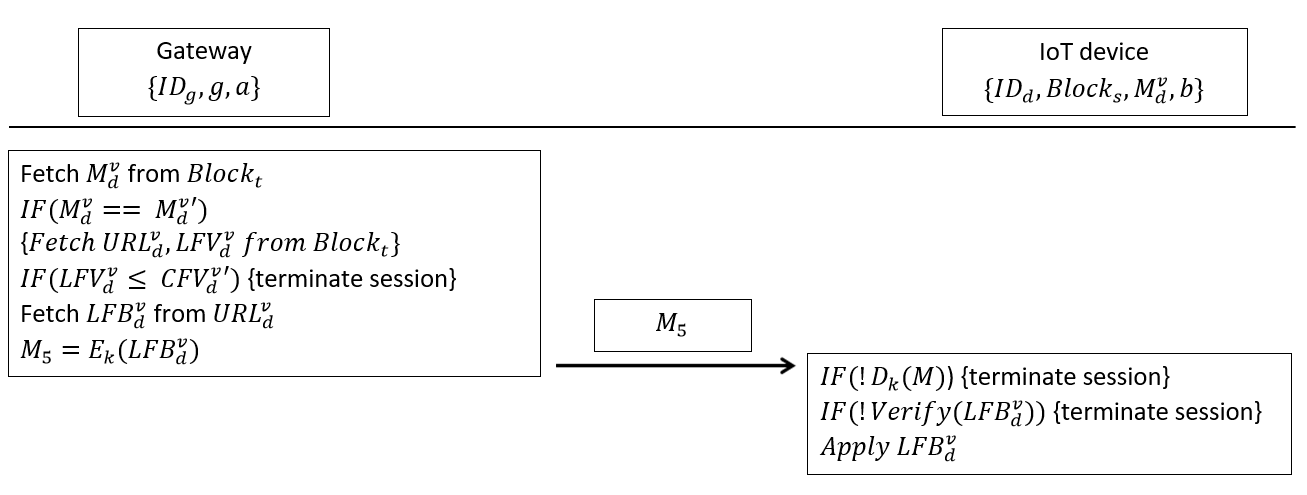
\includegraphics[width=1.0\textwidth]{figures/firmware_update_execution_2.png}
		\caption{Firmware update execution protocol} 
		\label{fig:executionprocessprotocol}
	\end{center}
\end{figure}

\noindent \underline{\textbf{Step 1:}} $\text{Gateway}\rightarrow\text{IoT Device}$ \\
\indent Gateway will fetch the target device model $M_d^v$ from the newly created block $BLOCK_t$. It will check if the targeted model device is same as the IoT device model $M_d^{v'}$ belonging to it. If there is targeted device model within its belonging IoT device ($M_d^v == M_d^{v'}$), it will fetch the download url $URL_d^v$ and the latest firmware version $LFV_d^v$ from the block $BLOCK_t$. Gateway will check if the latest firmware version is greater than the device current firmware version ($LFV_d^v \geq CFV_d^{v'}$). If the update is required, gateway will fetch the firmware binary $LFB_d^v$ from the download url $URL_d^v$. Last, gateway encrypt message $m_5=E_k(LFB_d^v)$ using session key $k$, then send the message $m_5$ to IoT device.

\noindent \underline{\textbf{Step 2:}} $\text{IoT Device}\rightarrow\text{Gateway}$ \\
\indent IoT device will decrypt the encrypted message \textit{$m_5'$} using its session key \textit{$k$}, and obtain the new firmware update binary. IoT device will verify the obtained \textit{$LFB_d^{v'}$} using its pre-installed vendor's public key. Once verified, IoT device will execute the firmware binary \textit{$LFB_d^{v'}$} and do the update process.
	% \chapter{Prototype Design and Implementation}
\label{cha:4_prototypeImplementation}
\parskip=0ex
This chapter describes prototype design of our proposed skipchain-based firmware update framework in Section~\ref{sec:prototypedesign}. The implementation of the proposed framework and the result of the experiments described in Section~\ref{sec:prototypeimplementation}. 

\section{Prototype Design}
\label{sec:prototypedesign}

This section describe two main procedures used in the prototype implementation. First, the key exchange procedure is described in Subsection~\ref{subsec:keyexchange}. Second, encryption and decryption procedures are described in Subsection~\ref{subsec:aes_enc} and Subsection~\ref{subsec:aes_dec} respectively.

\subsection{Key Exchange Procedure}
\label{subsec:keyexchange}

We have implemented two type of prototypes with two different involved parties. The first prototype design (called the repository-node prototype) simulates protocol between vendor repository as a client and vendor node as a server, this prototype uses the Internet as the information exchange connection protocol. Second prototype (called the gateway-IoT device prototype) implements client-server architecture between gateway and IoT device. The second prototype uses Bluetooth connection to exchange the information. The gateway takes the role of Bluetooth server and the IoT device takes role of Bluetooth client.

\sloppy Both prototypes use Diffie-Hellman~\cite{Diffie:2006:NDC:2263321.2269104} key exchange protocol. The three stages of key exchange protocol are described in Algorithm \ref{client_algo},\ref{server_algo},\ref{client_algo2}. In initiation procedure from Algorithm \ref{client_algo}, \textbf{vendor repository} (in repository-node prototype) uses $WIFI\_CLIENT\_SOCKET$ and \textbf{IoT device} (in gateway-device prototype) uses $BLUETOOTH\_CLIENT\_SOCKET$. The client sets some pre-defined variables used in key exchange procedure. After the pre-setting is complete, the client concatenates the variables as one string message. The message will be concatenated with its hashed-value and send via $CLIENT\_SOCKET$ to the server.

\begin{algorithm}[H]
	\caption{Client Key Exchange Initiation}\label{client_algo}
	\begin{algorithmic}[1]
		\Procedure{Key\_Exchange\_Procedure\_Client}{}
		\State $SERVER\_ADDRESS:140.118.109.81$
		\State $INIT\ CLIENT\_SOCKET(HOST:140.118.109.81,PORT:8080)$
		\State $SET\ ID_v:"vendorA\_repo\_1"$
		\State $SET\ a:6 \gets secret\_number$
		\State $SET\ g:5 \gets shared\_base$
		\State $SET\ p:RANDOM() \gets random\ shared\_prime$
		\State $SET\ sid:TODAY()$
		\State $CALCULATE\ A=g^amod(p)$
		\State $m=(sid||ID_v||g||p||A) \gets message$
		\State $CLIENT\_SOCKET.SEND(m||SHA256(m))$
		\EndProcedure
	\end{algorithmic}
\end{algorithm}

The response for Algorithm ~\ref{client_algo} is described in Algorithm \ref{server_algo}. In the response procedure, \textbf{vendor node} (in repository-node prototype) uses $WIFI\_SERVER\_SOCKET$ and \textbf{gateway} (in gateway-device prototype) uses $BLUETOOTH\_SERVER\_SOCKET$. $SERVER\_SOCKET$ to receive the message from client. The server fetch the concatenated message by using split function. 

After applying the split function to the message, the server gets an array value. If the array length does not match the required length in the procedure (6), the server will terminate the session. Otherwise, server put each array component into different variables. The server will check if the hashed-value in the last array component matches with the hashed-value of newly created variables.

Once the message is verified, the server calculates the shared secret $s$ and uses PBKDF2 \cite{wiki:pbkdf2}. PBKDF2 function is a key derivation function that applies hash-based message authentication code (HMAC) to the input passphrase ($s$) along with a salt value ($sid$). The derivative function repeats many times to produce a derived key, the key can be used as a cryptographic key in subsequent operations. Cryptographic key produced from KDF will be the session key for AES encryption-decryption key in Algorithm \ref{aes_enc},\ref{aes_dec}.

The last step in the server-side is sending the required data $B$, that is used for the $SHARED\_SECRET$ creation in the client-side. Server concatenates the message and its hashed-value, then send it to the client. Key exchange procedure in server-side is ended here, and the server has acquired the shared secret $s$.

\begin{algorithm}[H]
	\caption{Server Key Exchange Response}\label{server_algo}
	\begin{algorithmic}[1]
		\Procedure{Key\_Exchange\_Procedure\_Server}{}
		\State $INIT\ SERVER\_SOCKET(HOST:127.0.0.1,PORT:8080)$
		\State $SET\ ID_c:"id\_vendorA\_cothority\_1"$
		\State $SET\ b:15 \gets SECRET\_NUMBER$
		\State $SERVER\_SOCKET.LISTEN(1)$
		\State $DATA = SERVER\_SOCKET.RECEIVE(1)$
		\If {$(DATA.LENGTH() > 0)$} 
		\State $ARRAY\_DATA = DATA.SPLIT()$
		\If{$(ARRAY\_DATA.LENGTH()\ != 6)$}
		\State $TERMINATE\_SESSION()$
		\EndIf
		\State $SET\ sid'=ARRAY\_DATA[0]$
		\State $SET\ ID_v'=ARRAY\_DATA[1]$
		\State $SET\ g'=ARRAY\_DATA[2] \gets shared\ base$
		\State $SET\ p'=ARRAY\_DATA[3] \gets shared\ prime$
		\State $SET\ A'=ARRAY\_DATA[4] \gets shared\ number$
		\State $SET\ hash\_value'=ARRAY\_DATA[5]$
		\If{$(SHA256(sid'||ID_v'||g'||p'||A')\ == hash\_value')$}
		\State $s=A'^{(b)}mod(p') \gets shared\ secret$
		\State $k=PBKDF2(s,sid') \gets session\ key$
		\State $B=g'^{(b)}mod(p') \gets shared\ number$
		\State $m=(sid'||ID_c||B) \gets message$
		\State $SERVER\_SOCKET.SEND(m||SHA256.H(m))$
		\EndIf
		\Else
		\State $TERMINATE\_SESSION()$
		\EndIf
		\EndProcedure
	\end{algorithmic}
\end{algorithm}

The last procedure in the client-side is described in Algorithm~\ref{client_algo2}. In the first step, the client splits the response message from the server. If the array length matched the required length (4), the client put each array component into different variables then runs verification process to check if the hashed-value in the last array component matches with the hashed-value of newly created variables. If the message is verified, the client calculates the shared secret uses the shared number $B$. In the last step, the client uses PBKDF2 to produce same session key as the server owns.


\begin{algorithm}[H]
	\caption{Client Key Exchange End}\label{client_algo2}
	\begin{algorithmic}[1]
		\Procedure{Key\_Exchange\_Procedure\_Client}{}
		\State $SERVER\_ADDRESS:140.118.109.81$
		\State $INIT\ CLIENT\_SOCKET(HOST:140.118.109.81,PORT:8080)$
		\State $DATA = CLIENT\_SOCKET.RECEIVE(1)$
		\If {$(DATA.LENGTH() > 0)$} 
		\State $ARRAY\_DATA = DATA.SPLIT()$
		\If{$(ARRAY\_DATA.LENGTH()\ != 4)$}
		\State $TERMINATE\_SESSION()$
		\EndIf
		\State $SET\ sid'=ARRAY\_DATA[0]$
		\State $SET\ ID_c'=ARRAY\_DATA[1]$
		\State $SET\ B'=ARRAY\_DATA[2] \gets shared\ number$
		\State $SET\ hash\_value'=ARRAY\_DATA[3]$
		\If{$(SHA256(sid'||ID_c'||B')\ == hash\_value')$}
		\State $s=B'^{(a)}mod(p') \gets shared\ secret$
		\State $k=PBKDF2(s,sid') \gets session\ key$
		\EndIf
		\Else
		\State $TERMINATE\_SESSION()$
		\EndIf
		\EndProcedure
	\end{algorithmic}
\end{algorithm}


\subsection{AES Encryption Function}
\label{subsec:aes_enc}

After both the client and the server have the same session key, they can use the session key as AES symmetric key. Client and server use the AES encryption architecture to send sensitive information. AES encryption function described in Algorithm \ref{aes_enc}. The encryptor need to prepare a symmetric key $k$ to create an AES object. The encryptor uses session id $sid$ as salt and generate nonce value $IV$. The function encrypts the plain text using the nonce $IV$, then concates the hex-value of the result with the hex-value of the salt and the nonce ($HEX(SALT)||HEX(IV)||HEX(AES\_RESULT)$)

\begin{algorithm}[H]
	\caption{AES Encryption Function}\label{aes_enc}
	\begin{algorithmic}[1]
		\Procedure{AES\_Encryption}{}
		\State $GET\ sid', k \gets defined\ in\ algorithm\ \ref{client_algo2}$
		\State $INIT\ AES\_ = AESGCM(k)$
		\State $INIT\ IV = RANDOM() \gets nonce\ value$
		\State $INIT\ SALT = sid'$
		\State $INIT\ PLAINTEXT = "this\ is\ message"$
		\State $\#None\ associated\_data\ need\ to\ be\ authenticated$
		\State $SET\ AES\_RESULT = AES\_.ENC(IV,PLAINTEXT,None) $
		\State $SET\ CIPHER = HEX(SALT)||HEX(IV)||HEX(AES\_RESULT)$
		\State $RETURN\ CIPHER$
		\EndProcedure
	\end{algorithmic}
\end{algorithm}

\subsection{AES Decryption Function}
\label{subsec:aes_dec}

By using the same symmetric key $k$, the other party can decrypt the cipher text that created using Algorithm \ref{aes_enc}. The AES decryption fucntion is described in Algorithm \ref{aes_dec}. In the first step, the decryptor creates same AES object as encryptor using session key $k$. The decryptor splits the received cipher text, then decode the cipher text using $UNHEX()$ function. Afterward, the decryptor removes the salt from the decoded cipher text and uses the decryption function from the AES object to decrypt the decoded cipher text. The decryption function $AES\_.DEC()$ requires the nonce value ($IV$) and the decoded cipher text and return the plain text as result.

\begin{algorithm}[H]
	\caption{AES Decryption Function}\label{aes_dec}
	\begin{algorithmic}[1]
		\Procedure{AES\_Decryption}{}
		\State $GET\ k \gets defined\ in\ algorithm\ \ref{client_algo2}$
		\State $GET\ CIPHER' \gets defined\ in\ algorithm\ \ref{aes_enc}$
		\State $INIT\ AES\_ = AESGCM(k)$
		\State $SET\ SALT',IV',CIPHER\_TEXT' = UNHEX(CIPHER'.SPLIT())$
		\State $INIT\ PLAINTEXT = AES\_.DEC(IV,CIPHER\_TEXT,None)$
		\State $RETURN\ PLAINTEXT$
		\EndProcedure
	\end{algorithmic}
\end{algorithm}

\section{Prototype Implementation}
\label{sec:prototypeimplementation}

For our prototype implementation, we use the following devices:
\begin{table}[H]
	\caption{The device specification for each role}
	\label{tab:devicespec}
	\begin{center}
		\begin{tabular}{|l|l|}
			\hline
			\textbf{Roles} & \textbf{Device} \\ \hline
			\textbf{IoT Device} & \begin{tabular}{l@{}l@{}l@{}l@{}}  \textbf{Raspberry Pi 3} with the following specification: \\ - CPU: ARM Cortex 1,4GHz \\ - RAM: 1GB SRAM \\ - Bluetooth version: 4.0\end{tabular} \\ \hline
			\textbf{Vendor Repository} & \begin{tabular}{l@{}l@{}l@{}l@{}l@{}}  \textbf{MSI GL62 laptop} with the following specification: \\ - CPU: Intel i7 2,6GHz \\ - RAM: 16GB \\ - SSD: 512GB \\ - Bluetooth version: 4.0\end{tabular} \\ \hline
			\textbf{ Vendor Node and Gateway} & \begin{tabular}{l@{}l@{}l@{}l@{}}  \textbf{Asus PC} with the following specification: \\ - CPU: Intel i5 2,3GHz \\ - RAM: 12GB  \\ - Bluetooth version: 4.0\end{tabular} \\
			\hline
		\end{tabular}
	\end{center}
\end{table}
%\begin{enumerate}
%	\item MSI GL62 laptop as vendor repository equipped with Intel i7 2,6GHz, 16 GB RAM, SSD 512MB.
%	\item Asus PC as vendor node and gateway equipped with Intel i5 2,3GHz, 12 GB RAM, HDD, and Bluetooth 4.0 dongle. This PC run 4 virtual device as active node and 1 virtual device as passive node (gateway function) to simulate the skipchain environment.
%	\item Raspberry Pi 3 as IoT device, equipped with CPU: ARM Cortex 1,4GHz, 1GB SRAM, Integrated Bluetooth 4.0.
%\end{enumerate}
We use Python as programming language and run the python script in each device. The skipchain node within the network is created using the github code from the Chainiac paper \cite{chainiac}. As the open source code for the skipchain is still under hard development, we could not find a more suitable API by the time of this thesis writing. As a result, we use python library (\textbf{subprocess}) to access the skipchain via terminal. 

We conduct two experiments on the implemented prototype as follow:
\begin{enumerate}
	\item First, we perform experiment between vendor repository and vendor node using the Internet connection. The average running time after running the first experiment 10 times is one second. The process of putting the data to the skipchain takes $90\%$ of the running time.
	\item Second, we conduct experiment between gateway and IoT device using Bluetooth connection. Average running time after running the second experiment 10 times is one second. It takes 50 microseconds to send 10 megabytes of firmware data over the Bluetooth connection.
\end{enumerate} 
	% \chapter{Security and Performance Analyses}
\label{cha:5_analysis}
\parskip=0ex

In this chapter, security analysis of the proposed firmware update framework and protocol are provided and discussed. There is security analysis against attack within information exchange over insecure connection described in Section~\ref{sec:securityOverInsecure}. In the Section \ref{sec:protocolAnalysisTool} discussed how we use the analysis tools and the result. Performance analysis also conducted in Section~\ref{sec:performance} to compare the performance of the proposed protocol against existing firmware update protocol. In last section, Section~\ref{sec:discussion} summary the security analysis result from the previous sections.

% \begin{tabular}{@{}c@{}}\textbf{Peer-to-peer} \\ \textbf{firmware file sharing}\end{tabular}

\begin{table}[htb]
	\caption{Architecture design comparison of four blockchain-based firmware update framework}
	\label{tab:architectureComparison}
	\begin{adjustbox}{max width=1\textwidth,center}
		\begin{tabular}{|l|l|l|l|l|}
			\hline
			\textbf{Architecture design} & \textbf{Proposed framework} & \textbf{Yohan et al.~\cite{yohan}} & \textbf{Lee et al.~\cite{lee}} & \textbf{Boudguiga et al.~\cite{lee}}\\ \hline
			\textbf{Firmware update method} & Push-method & Push-method & Pull-method & Pull-method\\ \hline
			\textbf{Vendor platform} & Multiple vendors & Multiple vendors & Single vendor & Multiple vendors\\ \hline
			\textbf{IoT device platform} & Heterogeneous devices & Heterogeneous devices & Specific device & Heterogeneous devices\\ \hline
			\begin{tabular}{@{}l@{}}\textbf{Peer-to-peer firmware} \\ \textbf{ file sharing}\end{tabular} & Not allowed & Not allowed & Allowed & Allowed\\ \hline
			\textbf{Blockchain platform} & Skipchain & Ethereum & Bitcoin & Bitcoin\\ \hline
			\textbf{Smart Contract} & Available & Available & Not available & Not available\\ \hline
			\textbf{Trusted node} & Not-required & Not-required & Not-required & Required\\ \hline
			\textbf{Peer-to-peer verification} & Yes & No & No & No\\ \hline
		\end{tabular}
	\end{adjustbox}
\end{table}

Our proposed framework uses push-method to distribute the updated firmware, where a vendor can publish an update and notify the targetted device within the blockchain network without specific request from the device. The other two blockchain-based firmware achitectures~\cite{lee,boudguiga} applied pull-method, where an IoT device needs to send a firmware update request to check for the new available firmware version. Push-method can reduce attack-window time by updating the firmware immediately after the vendor publishes a new firmware update. Push-method is also more energy and network efficient than pull-method, because in pull-method, power-constrained and connection-limited IoT devices need to constantly request the availability of the new firmware version whether it is exist or not.

Our framework achitecture adopts skipchain technology, which enables smart contract creation. Skipchain as permissioned blockchain platform protocols adapts PBFT concept in the consensus mechanism. In our proposed framework, PBFT is a better choice because the framework does not allow anyone to join the blockchain network but only for registered vendor and gateway. PBFT tackle the energy required by proof-of-work consensus mechanism with drawback of no anonimity within the permissioned blockchain network.

Our proposed framework is able to provide peer-to-peer skipblock verification process by using the skipchain technology's forward link. It means that low-power with little or no Internet connectivity device does not need to maintain connections with many other network nodes. Low-power device can get the up-to-date block data from the stronger device (e.g gateway) via peer-to-peer connection, and securely verify if the new block data is exist in the valid skipchain network without storing the whole blockchain data.

\begin{table}[htb]
	\caption{The comparison of security mechanism against cyber attack of four blockchain-based firmware update framework}
	\label{tab:securityComparison}
	\begin{adjustbox}{max width=1\textwidth,center}
		\begin{tabular}{|l|l|l|l|l|}
			\hline
			\textbf{Provide protection against} & \textbf{Proposed framework} & \textbf{Yohan et al.~\cite{yohan}} & \textbf{Lee et al.~\cite{lee}} & \textbf{Boudguiga et al.~\cite{lee}}\\ \hline
			\textbf{Firmware modification attack} & Yes & Yes & No & Yes\\ \hline
			\textbf{Impersonation attack} & Yes & Yes & No & Yes\\ \hline
			\textbf{Man-in-the-middle attack} & Yes & Yes & Yes & Not specified\\ \hline
			\textbf{Replay attack} & Yes & Yes & Yes & Not specified\\ \hline
			\textbf{Isolation attack} & Yes & No & No & No\\ \hline
		\end{tabular}
	\end{adjustbox}
\end{table}

The comparison of the security mechanism between proposed framework and the other related works is shown in Table~\ref{tab:securityComparison}. Our proposed framework is designed to protect the firmware update process from major cyber-attack, respectively: firmware modification attack, impersonation attack, man-in-the-middle attack, replay attack and isolation attack. On the other hand, the firmware update mechanism proposed by Lee et al.~\cite{lee} could not prevent firmware modification and impersonation attack. Furthermore, our proposed framework provides additional security measure against isolation attack.

By nature, an offline blockchain node can not resist isolation attack, because there is no cryptographic means for any node to distinguish the real blockchain from a fake one. If an attacker can isolate (even temporarily) a node from the network, attacker can tricks the isolated node to accept the fake firmware update from newer block that never exist.

\section{Informal Security Analysis} 
\label{sec:securityOverInsecure}

The following theorems are applied on both firmware verification protocol and peer-to-peer verification protocol. \textbf{Vendor repository} roles in firmware verification protocol and \textbf{IoT devices} roles in peer-to-peer verification protocol act as \textit{client} in the theorems. \textbf{Vendor node} roles in firmware verification protocol and \textbf{gateway} roles in peer-to-peer verification protocol act as \textit{server} in the theorems. The theorems are under assumption that the cryptographic hash function used in the proposed framework is assumed to be able to withstand all known types of cryptanalytic attacks. This means the hash function has the capability of collision resistance, counteracts preimage attacks and second-preimage attacks.

In addition, the proposed protocol assumed to use a Cryptographically Secure Pseudorandom Number Generator (CSPRNG). CSPRNG must satisfied all statistical test and need to be unpredictable, means attacker unable to predict the next output of random value. Based on these assumption and annotations, the security analysis of the proposed protocol is defined as follow:
\renewcommand{\qedsymbol}{}
\newtheorem{theorem}{Theorem}
\begin{theorem}
	\label{theo:mutualAuth}
	The proposed protocol supports mutual authentication and data integrity
\end{theorem}
\begin{proof}
	Because of the computational difficulty to collect shared secret from Diffie-Hellman key exchange protocol, only legitimate client and server can calculate the secret. Client uses the shared public key $B$ from the server and its private key $a$, calculate $s = B^amod(p)$. On the other hand, server uses the shared public key $A$ from client and its private key $b$, to calculate the same shared secret $s = A^bmod(p)$. Client and server then use the shared secret $s$ and session id $sid$ to create session key $k=KDF(s,sid)$. Adversary who collects public material from the key exchange protocol will not be able to produce the same shared secret $s$ without the private key $(a,b)$.\\
	\indent Furthermore, legitimate client and server can verify the hashed-value message from each other using predefined hash-chain function $H()$. Adversary who does not know the hash-chain function, will not be able to re-create the same hashed-value message and send it to the client or server. For example, if client send a message $M_1 = m_1||H(m_1)$ to the server. Server can use the same hash-chain function $H()$ and authenticate if the message comes from client, vice-versa $H(m_1')==H(m_1)'$.Based on these two proofs, it can be concluded that the proposed protocol supports mutual authentication and data integrity.
\end{proof}

\begin{theorem}
	The proposed protocol supports session key security
\end{theorem}
\begin{proof}
	In proposed protocol, both client and server always use newly generated shared prime $p$ in key exchange protocol and session id $sid$ as salt in session key $k$ generation. The adversary needs to solve the Diffie-Hellman problem to get the current shared secret $s$ and use the same key derivation function $KDF()$ as a client and server uses to get the current session key $k$. Because it is difficult to solve computational problem of Diffie-Hellman, and also hard to find accurate key derivation function $KDF()$, the proposed protocol provides session key security. This also proves that the protocol is able to defense against forward secrecy attack.
\end{proof}

\begin{theorem}
	The proposed protocol defends against impersonation attack
\end{theorem}
\begin{proof}
	There are three targets for the adversary to impersonates to, namely: vendor repository, vendor node, and gateway. First, adversary can try to impersonate to a vendor repository and send invalid firmware update metadata to the vendor node. In order to deceive the vendor node, it need to send the message and its hashed-value to complete the authentication protocol. It is difficult to find the exact hash-chain function $H()$ using brute force, because after failing a session, server or client will catch the sender ip or mac address and blacklist the address if it fail up-to certain threshold. Additionally, adversary needs to get the vendor repository private key to sign the metadata. Because later, the metadata will be verified by the cothority member before put into the skipchain.\\
	\indent Second, adversary can try to impersonate to a vendor node and deceive the cothority's member to sign malicious contract and put into skipchain network. Adversary need to join the permission blockchain platform as cothority's member. Because the cothority's member is predefined before the skipchain creation and the member's change need to be verified by the threshold of other member. It is presumably hard if adversary does not control more than one third of the cothority member.\\
	\indent Third, adversary can try to impersonate to a gateway and deceive IoT device that there is new fake firmware update. The forward link in skipchain enables IoT device to verify the new block that contain new firmware update in the peer-to-peer connection. In order to create fake block, adversary need to have a threshold of cothority member's private key and sign the fake block with it. This attack is not plausible, especially if the cothority member is changing overtime. Hence, it could be concluded that the proposed protocol defends against impersonation attack.\\
\end{proof}

\begin{theorem}
	The proposed protocol defends against replay attack
\end{theorem}
\begin{proof}
	Assuming that adversary tries to perform replay attack on the proposed protocol, both firmware verification and peer-to-peer verification protocol. Adversary can send the collected valid-message $M_1$ from the previous session and replays the transaction repeatedly to cause an unnecessary transactions. However, our proposed protocol uses timestamped session id $sid$, so when an obsolete transaction is detected, it will be rejected and the session will be terminated. If an address failing session up-to certain threshold, it will be blacklisted from the server or client.\\
	\indent In addition, skipchain mechanism does not allow duplicate timestamped transaction. The duplicate transaction will be dropped during the validation process by cothority's member. Therefore, it is concluded that replay attack does not affect our proposed framework
\end{proof}

\begin{theorem}
	\label{theo:mitm}
	The proposed protocol defends against man-in-the-middle attack
\end{theorem}
\begin{proof}
	Based on the proof given for Theorem~\ref{theo:mutualAuth}, proposed protocol provides mutual authentication between legitimate client and legitimate server. In addition, adversary can not use the session key $k$ to decrypt and get the important metadata and the firmware binary during the process. Thus, proposed protocol keeps the secrecy of the important data. Hence, the proposed protocol defends against man-in-the-middle attack.
\end{proof}

\begin{theorem}
	The proposed protocol defends against firmware modification attack
\end{theorem}
\begin{proof}
	Based on the proof given for Theorem~\ref{theo:mutualAuth} and Theorem~\ref{theo:mitm}, proposed protocol provides mutual authentication and defends against man-in-the-middle attack. Furthermore, the firmware update contract contains firmware location $URL^v_d$. If an adversary aim to modify the firmware binary, adversary needs to aim non secure channel during the firmware binary transmission. And the only non secure channel is peer-to-peer connection between gateway and IoT device, since the gateway downloads the firmware binary from vendor repository using TLS secure channel. If somehow, adversary can modify the firmware binary and forward it, IoT device can detect the firmware binary is invalid. IoT device with pre-installed vendor's public key can verify the signed-firmware-binary.
\end{proof}

\section{Protocol Verification Using Scyther Tool} 
\label{sec:protocolAnalysisTool}

Scyther is a tool used for security protocol verification, where it is assumed that all the cryptographic functions are perfect. Scyther tool can find security problem that arise from the way the protocol is constructed. The language used to write proposed protocol structure in Scyther is SPDL. Our proposed protocol then validated using 'automatic claim' and 'verification claim' procedures in the Scyther tool. The result of each claim will be explained in the following subsection.

\begin{figure}[H]
	\begin{center}
		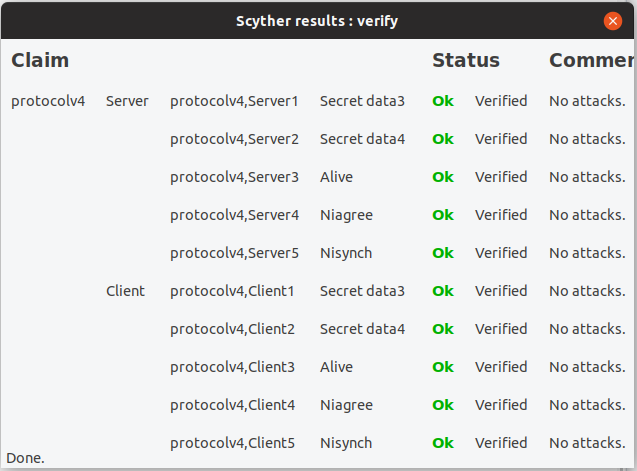
\includegraphics[width=1.0\textwidth]{figures/scyther-result.png}
		\caption{Scyther tool verification result} 
		\label{fig:scytherResult}
	\end{center}
\end{figure}

\subsection{Data Secrecy}

In the proposed protocol, sensitive information (denoted as \textit{data} in Figure~\ref{fig:scytherResult}) secrecy is achieved by encrypting each data using symmetric key $k$ algorithm which is shared between client (C) and server (S). In firmware verification protocol, vendor repository acts as a client and vendor node acts as a server. In peer-to-peer verification protocol, IoT device acts as a client and gateway acts as a server. The successful claim for the data secrecy is shown in Figure~\ref{fig:scytherResult}. The claim used in the SPDL code is:

\begin{table}[H]
	\begin{center}
		\begin{tabular}{l}
			\hline
			$\# server\ role$\\
			\boldmath{$claim(Server,Secret,data3)$} $\# server\ send\ data3$ \\
			\boldmath{$claim(Server,Secret,data4)$} $\# server\ receive\ data4$ \\
			$\# client\ role$\\
			\boldmath{$claim(Client,Secret,data3)$} $\# client\ receive\ data3$ \\
			\boldmath{$claim(Client,Secret,data4)$} $\# client\ send\ data4$ \\
			\hline
		\end{tabular}
	\end{center}
\end{table}

\subsection{Aliveness}

In the Figure~\ref{fig:scytherResult}, proposed protocol claims to ensure the server and client liveliness during the information transmission. The claim used in the SPDL code is:

\begin{table}[H]
	\begin{center}
		\begin{tabular}{l}
			\hline
			$\# server\ role$\\
			\boldmath{$claim(Server,Alive)$}\\
			$\# client\ role$\\
			\boldmath{$claim(Client,Alive)$} \\
			\hline
		\end{tabular}
	\end{center}
\end{table}

\subsection{Non-injective Agreement and Non-injective Synchronisation}

In the Figure~\ref{fig:scytherResult}, proposed protocol claims to ensure non-injective agreement and non-injective synchronisation during the information transmission. Based on \cite{nisyncandnyaggre}, non-injective agreement means all variables sent as part of the message $m$ are received as expected. Therefore, both parties will agree over the values of the variables that are sent. Non-injective syncronisation means the send event from the first run \textit{send\_1} followed by corresponding read \textit{recv\_1} and so on until the send-read event in the end of the protocol. The claim used in the SPDL code is:

\begin{table}[H]
	\begin{center}
		\begin{tabular}{l}
			\hline
			$\# server\ role$\\
			\boldmath{$claim(Server,Niagree)$}\\
			\boldmath{$claim(Server,Nisynch)$}\\
			$\# client\ role$\\
			\boldmath{$claim(Client,Niagree)$}\\
			\boldmath{$claim(Client,Nisynch)$}\\
			\hline
		\end{tabular}
	\end{center}
\end{table}

\section{Performance Analysis} 
\label{sec:performance}

In this section, comparison on performance between the proposed firmware update protocol and existing firmware update protocol are discussed. Table~\ref{tab:performanceComparison} shows the comparison of time consumption to do firmware verification protocol and peer-to-peer verification protocol between the proposed protocol and three existing firmware update protocol \cite{yohan,lee,boudguiga}.

In order to compare the computation cost between the proposed firmware update protocol and the existing protocol, the following assumptions are applied:
\begin{enumerate}
	\item The size for session key $k$ in our proposed protocol is 256 bits
	\item The symmetric encryption and decryption operation uses AES GCM with 256 bits key
	\item The one way hash function uses SHA256
	\item The key derivation function uses PBKDF2 with 1000 iterations in our proposed protocol, the output is session key $k$
\end{enumerate}
% \begin{tabular}{@{}c@{}}The time required to perform encryption (Enc) and decryption (Dec) \\ operations in symmetric cryptosystem\end{tabular}

\begin{table}[H]
	\caption{The performance comparison of four blockchain-based firmware update framework}
	\label{tab:performanceComparison}
	\begin{adjustbox}{max width=1\textwidth,center}
		\begin{tabular}{|l|l|l|}
			\hline
			\textbf{ } & \textbf{Firmware verification} & \textbf{Peer-to-peer verification} \\ \hline
			\textbf{Proposed framework} & $3T_H+2T_{KDF}+T_{symm\_enc}+T_{symm\_dec}$ & $4T_H+2T_{KDF}+3T_{symm\_enc}+3T_{symm\_dec}$\\ \hline
			\textbf{Yohan et al.~\cite{yohan}} & $6T_{sig}$ & $2T_{sig}+7T_{H}$\\ \hline
			\textbf{Lee et al.~\cite{lee}} & \begin{tabular}{@{}c@{}}$3T_{symm\_enc}+3T_{symm\_dec}+3T_{KDF}+$ \\ $10T_H+4T_{sig}$\end{tabular} & Not available \\ \hline
			\textbf{Boudguiga et al.~\cite{boudguiga}} & Not available & $4T_{sig}+T_{asymm\_enc}+T_{asymm\_dec}$ \\ \hline
		\end{tabular}
	\end{adjustbox}
\end{table}

\begin{table}[H]
	\caption{Notations used for time consumption on differing computing operations}
	\label{tab:notationtimeconsumption}
	\begin{adjustbox}{max width=1\textwidth,center}
		\begin{tabular}{cl}
			\hline
			\textbf{Notation} & \multicolumn{1}{c}{\textbf{Definition}} \\ \hline
			\boldmath{$T_H$} & The time required to perform one way hash function \\
			\boldmath{$T_{KDF}$} & The time required to perform key derivation function \\
			\boldmath{$T_{sig}$} & The time required to perform digital signature operation\\
			\boldmath{$T_{symm\_enc}$ and $T_{symm\_dec}$} & The time required to perform encryption (Enc) and decryption (Dec) operations in symmetric cryptosystem \\
			\boldmath{$T_{asymm\_enc}$ and $T_{asymm\_dec}$} & The time required to perform encryption (Enc) and decryption (Dec) operations
			in PKI cryptosystem \\
		\end{tabular}
	\end{adjustbox}
\end{table}

The execution time for the hash function (SHA256) and symmetric cryptographic operations (AES GCM) are calculated based on Crypto library benchmark using C++~\cite{cryptolib}. The benchmark compiled with Microsoft Visual C++ 2005 SP1, ran on Intel Core 2 1.83 GHz processor under Windows Vista in 32-bit mode. The execution time for the digital signature scheme and asymmetric operation (ECC 192-bits) are calculated based Yeh et al.~\cite{signatureScheme} and Tanwar et al.~\cite{asymmetricScheme}, repectively. The execution time for the cryptographic operations are shown in Table~\ref{tab:executionTime}. 

\begin{table}[H]
	\caption{The execution time of several cryptographic operations}
	\label{tab:executionTime}
	\begin{adjustbox}{max width=1\textwidth}
		\begin{tabular}{ll}
			\hline
			\textbf{Cryptographic operation} & \multicolumn{1}{c}{\textbf{Execution time}} \\ \hline
			SHA256 operation on 3200 bits of data & 28.8ms\\
			AES GCM symmetric encryption or decryption on 4000 bits of plain text & 39.21ms\\
			PBKDF2 with 1000 times iteration &  0.999ms\\
			Digital signature process (ECC 192-bits) & 11.52s \\
			ECC 192-bits asymmetric encryption or decryption & 1.064s \\
		\end{tabular}
	\end{adjustbox}
\end{table}

Based on Tabel~\ref{tab:performanceComparison}, the proposed protocol requires 166.818ms to finish firmware verification process ($3T_H+2T_{KDF}+T_{symm\_enc}+T_{symm\_dec}$). During the peer-to-peer verification process, the execution time for the proposed protocol is 352.458ms ($4T_H+2T_{KDF}+3T_{symm\_enc}+3T_{symm\_dec}$). In total, the execution time for the proposed protocol is 519.276ms.

On the contrary, the execution time of the firmware verification proposed by Lee et al.~\cite{lee} requires 46.606 seconds ($3T_{symm\_enc}+3T_{symm\_dec}+3T_{KDF}+10T_H+4T_{sig}$). Our proposed protocol has better performance regarding the execution time in the firmware verification process. The protocol proposed by~\cite{lee} requires more time to execute the digital signature process, including the digital signature verification process.

The execution time for  Yohan et al.~\cite{yohan} protocol of the firmware verification process is 69.12 seconds ($6T_{sig}$). For peer-to-peer verification,~\cite{yohan} need 23.2416 seconds, the protocol run time is 92.3616 seconds in total. Our proposed protocol also has better performance than~\cite{yohan} regarding execution time,~\cite{yohan} protocol required more time to execute the digital signature process.

The execution time for Boudguiga et al.~\cite{boudguiga} protocol of the peer-to-peer verification process is 48.208 seconds ($4T_{sig}+T_{asymm\_enc}+T_{asymm\_dec}$). Our proposed protocol has better performance than~\cite{boudguiga} regarding execution time, because~\cite{boudguiga} used digital signature and asymmetric cryptographic mechanism to secure their protocol.

\section{Discussion} 
\label{sec:discussion}

Our proposed framework leverages on the concept of skipchain to securely update the firmware in IoT environment. First, our proposed framework guarantee the secure sensitive information sharing during the process. Our proposed framework uses symmetric key algorithm to protect the sensitive information, the symmetric key algorithm uses session key produced from the shared secret from key sharing protocol. The symmetric key algorithm protects the sensitive data more computationally efficient than asymmetric key algorithm, which is more suitable for IoT environment. By using symmetric key algorithm it will also ensure the data integrity and privacy during the transmission process. Once the transaction is validated and recorded into the skipchain, this transaction can not be altered or deleted. Hence, our proposed framework could ensure end-to-end firmware integrity.

Second, our proposed framework uses skipchain, a permissioned blockchain platform, which only allows authorized vendor and gateway to join the skipchain network. Each time a vendor want to push a new firmware update, vendor need to sign the metadata with its private key. Later, the cothority member will verify the signature before put the metadata into the skipchain. Adversary can not impersonate a legitimate vendor and push a malicious firmware metadata into the skipchain, unless it has vendor's private key.

In addition, using of the long-distance backward link used in skipchain, vendor can rollback to previous firmware version efficiently if a problem occur in the new firmware (e.g. malfunction). Vendor can trace back previous stable firmware version, re-invoke the existing contract in the skipchain. It will notify the gateway to rollback based on the information in the re-invoked contract.

During the prototype implementation process, the open-source code in Github for skipchain is still under heavy development. Therefore, our prototype implementation could not use any API that calls the skipchain services. In the result, the prototype implementation uses command line interface to interact with the skipchain services. This could lead to performance issue, since we do not use direct API to call the skipchain service.

	% \chapter{Conclusions}
\label{cha:6_conclusions}

Firmware update is an essential process for vendor to manage its manufactured embedded device. Vendor can add new functionality, enchance security or re-configure the device through the new firmware update. Nowadays, automatic firmware update process is more commonly used, but the automatic process over the Internet is not without risk. Thus, a robust and lightweight protocol is needed to ensure the firmware security within the IoT environment. The proposed skipchain-based firmware update framework can enchance the end-to-end security of the firmware during the update process.

We investigate that using skipchain, a permission blockchain platform, can remove the traditional centralized architecture. Skipchain's forward link enables efficient peer-to-peer contract verification. This feature is important for offline embedded devices to verify the given contract without requires it to maintain connection with multiple nodes or storing any blockchain data. Thus, our contribution is provide perfect feature for low-power, connection restricted embedded device to verify the given firmware update contract.

Moreover, our proposed framework uses push method to keep the embedded device up-to-date as soon as the new firmware update release, which can shorten the vulnerable time. Our proposed framework is also proven to be secure and could withstand against firmware modification attack, impersonation attack, replay attack, man-in-the-middle attack, and isolation attack.

The improvement for our implementation can be made in the future works. By using the API to directly call the skipchain service, it is expected to shorten the protocol running time. It is also challenging to implement the peer-to-peer verification API, to verify a given contract.


	%----------------------------------------------------------------------------------------------------------------------------------------------------------
	% Back pages 後頁
	% Including: references, appendixes, and curriculum vitae
	% The structure of back pages for NTUST thesis is fixed,
	%	so do not alter the file ntust_backpages.tex structure whatsoever.
	% You can also comment out this back pages line while editing the main body of thesis.

	% 包括參考文獻、附錄、自傳
	% 實際內容由
	%    my_bib.bib, my_appendix.tex, my_vita.tex
	% 決定
	% ntust_backpages.tex 此檔只提供整體架構的定義,不需更動
	% 在撰寫各章草稿時,可以把此部份「關掉」,以節省無謂的編譯時間。

	%
% This file is encoded in utf-8
% v1.7
%

%%% References Document/ Bibliography 
\newpage
\addcontentsline{toc}{chapter}{\nameRef}
\renewcommand{\bibname}{\protect\makebox[5cm][s]{\nameRef}}		% '\makebox{}' is fragile, '\protect' will help
\bibliographystyle{ieeetr}										% Using IEEE Trans journal format
{\footnotesize
\bibliography{my_bib}  											% 'my_bib' is a BibTeX file located in the parent directory, it comprises all the references for the thesis
}

%%% Appendix (uncomment the following line to include the appendixes)
%%
% This file is encoded in utf-8
% v1.7
%

%%% Please copy the following TeX as the header code of each appendix (appendix 1, appendix 2, etc.):

%%% Header code begins >>>

\newpage
\chapter*{Appendix 1:MATLAB Source Code List} 							% Please change the values inside the curly brackets (the appendix number and the title)
\addcontentsline{toc}{chapter}{Appendix 1:MATLAB Source Code List} 	% It is recommended to set the same title as above
\renewcommand{\thechapter}{1} 											% if it is appendix 2, then it should be written as {2}

\setcounter{equation}{0} 
\setcounter{figure}{0} 
\setcounter{footnote}{0} 
\setcounter{section}{0} 
\setcounter{subsection}{0}
\setcounter{subsubsection}{0}
\setcounter{table}{0} 

%%% <<< Header code ends

% Appendix content is started from here

\lstinputlisting{example/example_prog_list.m}

%%% For generating appendix 2, 3, and so on, please continue by incrementing the order number in the TeX above
% Every appendix will automatically start as a new page

%%% Autobiography/ Vitae
%\newpage
%\chapter*{\protect\makebox[5cm][s]{\nameVitae}} 				% '\makebox{}' is fragile, '\protect' will help
%\addcontentsline{toc}{chapter}{\nameVitae}
%Fulan Chang is currently a Ph.D candidate 
in Department of Computer Science and Information Engineering 
from National Taiwan University of Science and Technology, Taipei, Taiwan. 
He received M.S degree in Department of Computer Science  and Information Engineering 
from National Taiwan University of Science and Technology in 2015. 
His current research interests include the Human-Computer Interaction, 
Tele-operation and Robotics. 



%%%%%%%%%%%%%%%%%%%%%%%%%%%%%%%%%%%%%%%%%%%%%%%%%%%%%%%%%%%%%%
%   Letter of Authorization (LoA/ 授權書)
%     ... the page numbers will be counted but not be printed
%%%%%%%%%%%%%%%%%%%%%%%%%%%%%%%%%%%%%%%%%%%%%%%%%%%%%%%%%%%%%%
%
% Insert the printed standard form when the thesis is ready to bind
% After the oral defense, put the LoA (signed by advisor) into the thesis, then bind it
% Create an entry in table of contents for this LoA
% Currently only generate an empty page

% Per January 2018, there is no need to include the copyright page
%   into the thesis book.
%   The copyright (authorization) letters are submitted separately to NTUST library.

%\newpage{\thispagestyle{empty}\addcontentsline{toc}{chapter}{\nameCopyrightForm}\mbox{}\clearpage}

%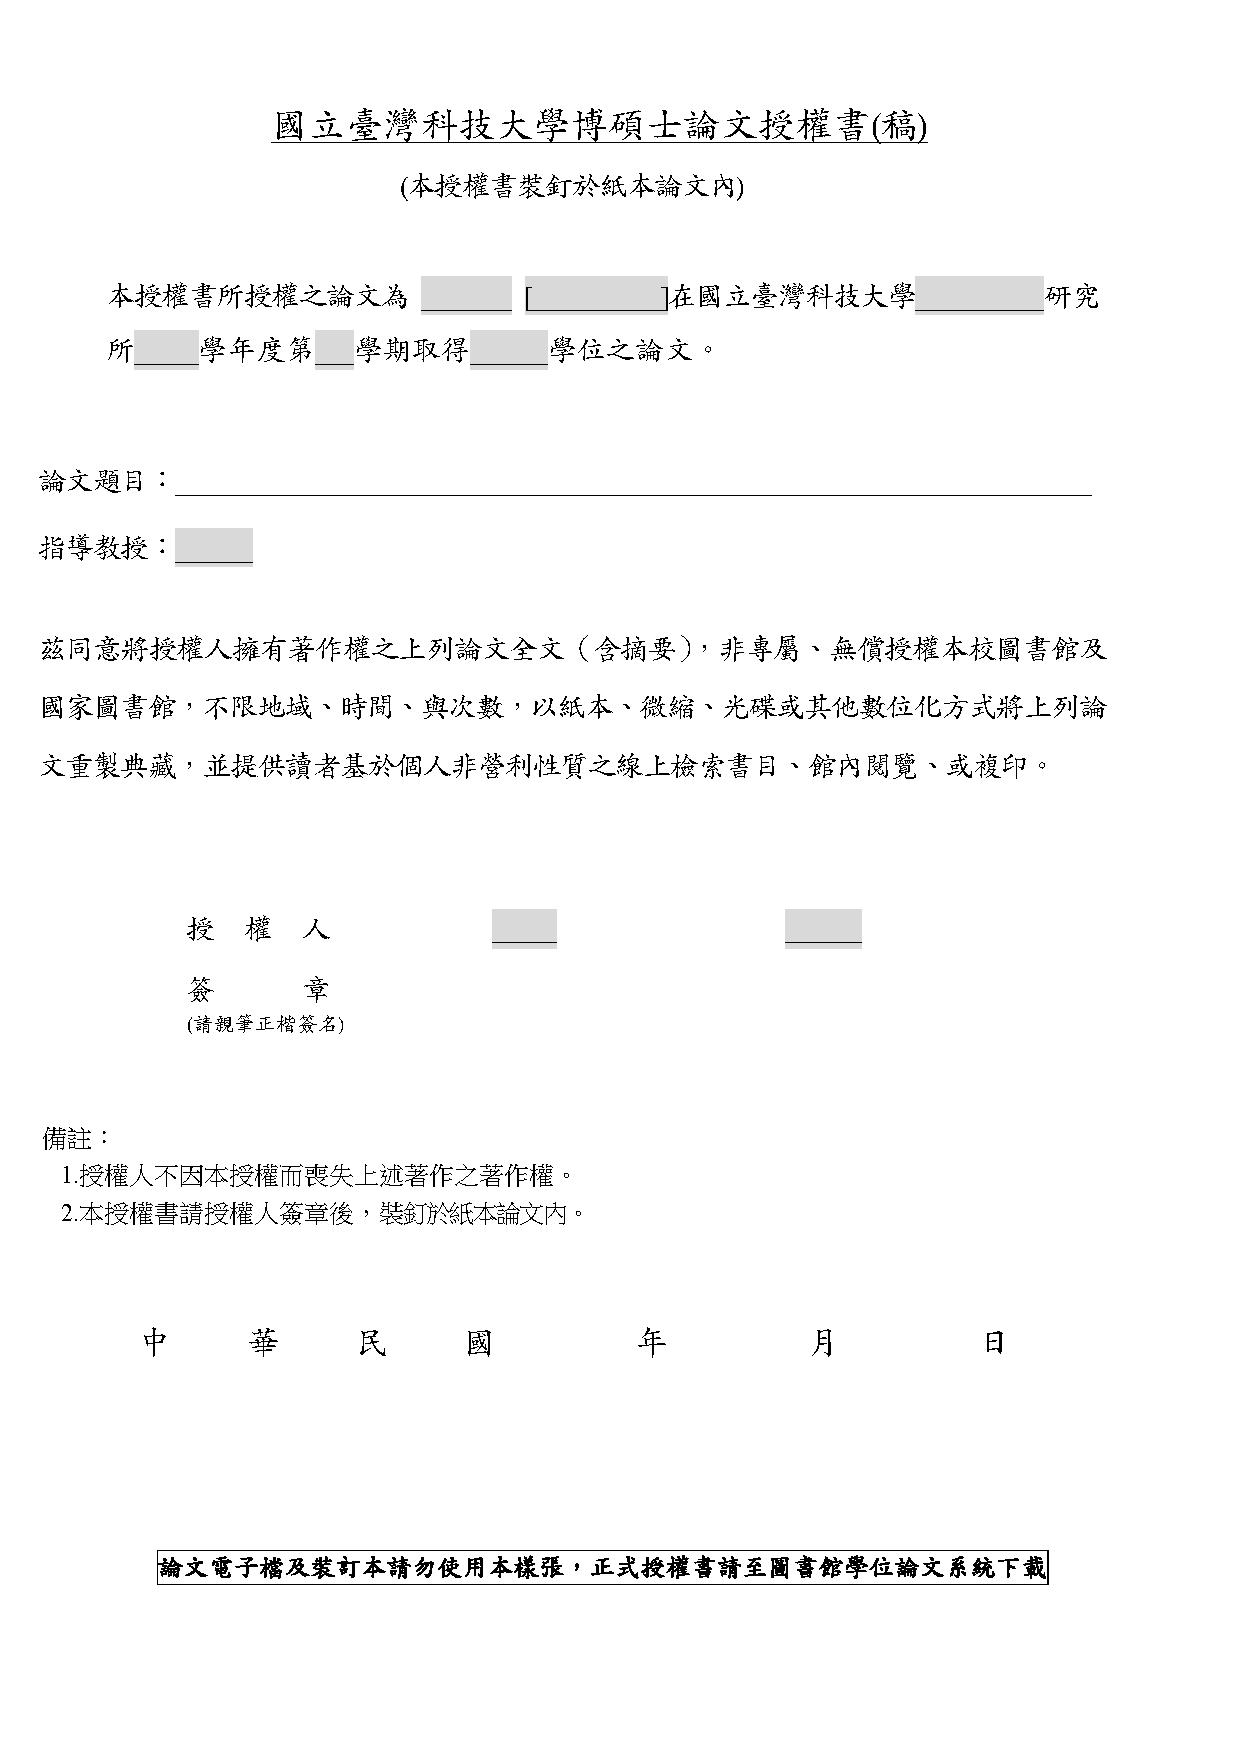
\includepdf{backpages/a.pdf}{\addcontentsline{toc}{chapter}{\nameCopyrightForm}}


%%%%% useless %%%%%
%\begin{figure}[!t]
%\centering
%\includegraphics[width=\paperwidth]{backpages/LetterofAuthority.pdf}
%\end{figure}
%\includepdf[addtotoc={1,chapter,-1,\nameCopyrightForm,letter}]{backpages/LetterofAuthority.pdf}
%\includepdf{backpages/LetterofAuthority.pdf}
%\addcontentsline{toc}{chapter}{\nameCopyrightForm}\mbox{}

\end{document} 
 
